% Sample Dissertation, Thesis, or Document %
%            for use with the              %
%  University of Arizona Thesis Class,     %
%               uathesis.cls               %
%------------------------------------------%

% We'll use the uathesis document class (duh).  The uncommented line
% below will produce a Dissertation, the others would produce a Thesis
% or a Document.  There are other options available to you like turning
% on the copyright statement and replacing the year on the title page
% with a "generated on" stamp (handy for early drafts).  To find out
% what the available options are, take a look into the uathesis.cls
% file and look for the \DeclareOption commands near the top of that
% file.
% There are five copyright options.  Copyright, no copyright, and three
% different Creative Commons licences.  Use the one you want (If you go
% Creative Commons, I (DM) think the CC-BY-ND makes the most sense)  See
% uathesis.cls for the reason why the non-commercial licenses are not
% included.
%\documentclass[dissertation]{uathesis}
%\documentclass[dissertation,copyright]{uathesis}
%\documentclass[dissertation,CC-BY]{uathesis}
%\documentclass[dissertation,CC-BY-SA]{uathesis}
\documentclass[dissertation,CC-BY-ND]{uathesis}
%\documentclass[dissertation,generatedon]{uathesis}
%\documentclass[thesis]{uathesis}
%\documentclass[document]{uathesis}

% Package Usage
% These are the packages that we need
%\usepackage{algorithm}
%\usepackage{algorithmic}
\usepackage[ruled,boxed,noend]{algorithm2e}
\usepackage{graphicx}
\usepackage{natbib}			% natbib is available on most systems, and is
					% terribly handy.
					% If you want to use a different Bibliography package, 
					% you should be able to, just change this
					% and the \bibliographystyle command below.  Be warned
					% that you may need to do a little hacking to get
					% the REFERENCES item to show up in your TOC.
\usepackage{latexsym}

\usepackage{amsmath}
\usepackage{fancyvrb, fancyhdr, theorem, latexsym, color, longtable}
\usepackage{multirow}
\usepackage{url}
\usepackage{bm}
\usepackage{amssymb}
\usepackage{fixltx2e}
\usepackage{tabularx}
%\usepackage{hyperref}

% Compatibility with the AASTEX package 
% of the American Astronomical Society.
%\usepackage{deluxetable}		% Allows use of AASTEX deluxe tables
%\usepackage{aastex_hack}		% Allows other AASTEX functionality.

% These are other packages that you might find useful.
% For controlling the fonts, see
% http://www.math.uiuc.edu/~hartke/computer/latex/survey/survey.html
% The following is a nice font set:
%\usepackage{mathtime}			% Times for letters; Belleek math.
%
%\usepackage{amsmath}			% AMS Math (advanced math typesetting)
%\usepackage{lscape}			% Used for making fitting large tables in by putting them landscape
%\usepackage{refs}			
%
% If you are using hyper-ref (recommended), this command must go after all 
% other package inclusions (from the hyperref package documentation).
% The purpose of hyperref is to make the PDF created extensively
% cross-referenced.
\usepackage[bookmarks,colorlinks=true,urlcolor=black,linkcolor=black,citecolor=black]{hyperref}


\usepackage{color}
\newcommand{\todo}[1]{\textcolor{red}{TODO: #1}}
\newcommand{\note}[1]{\textcolor{red}{#1}}
\newcommand{\svmr}{{SVM$^{rank}$}}
\newcommand{\code}[1]{{\tt {\small #1}}}
\newcommand{\qn}{{{\bf Q}$^\textbf{{\small N}}$}}
\newcommand{\ssa}{{{\scriptsize $^{*}$}}}

\DeclareMathOperator*{\argmax}{arg\,max}

% Set up some values.
\completetitle{My Lovely Dissertation}
\fullname{Rebecca Reynolds Sharp} % Grad college wants your full name here.
\degreename{Doctor of Philosophy}	% Title of your degree.

\begin{document}

% Set up the title page
\maketitlepage
{DEPARTMENT OF LINGUISTICS}	% Title of your department.
{2017}							

% Insert the approval form.  Note that for electronic submission
% of your Ph. D. dissertation, you must bring *two* copies of the
% approval page to your final defense.  These must be signed by
% the committee.  Make two photocopies: one for Pam and the other
% for your records.  Then, bring the two signed originals to the
% graduate college when you submit the final version of the
% dissertation to the University of Arizona.
\approval
{\textcolor{red}{11} August 2017}		% Defense Date	
{Michael Hammond}		% Dissertation Director
{Mihai Surdeanu}		% 2nd committee member
{Michael Hammond}		% 1st committee member
{Mihai Surdeanu}		% 2nd committee member
{Peter Jansen}		    % 3rd committee member
{} % 4th committee member (leave empty if None)

% Include the ``Statement by Author'' for Dissertations
\statementbyauthor
% If this is a Thesis, use the following form, with your thesis director's
% name and title in the square brackets like so (you should also omit the 
% approval form insertion above):
%\statementbyauthor[Jane M. Doe\\Professor of Chemistry]

% Include the ``Acknowledgements''
\incacknowledgements{acknowledgements}

% Include the ``Dedication''
\incdedication{dedication}

% Create a ``Table of Contents''
\tableofcontents

% Create a ``List of Figures''
\listoffigures

% Create a ``List of Tables''
\listoftables

% Include the ``Abstract''
\incabstract{abstract}

% Include the various chapters
\chapter{INTRODUCTION\label{chapter:introduction}}

\address{Start by explaining why NLI and QA are fundamental NLP tasks. Give examples to search, and personal assistants.}

\address{Natural language inference (NLI)}

\address{while FOL methods are attractive for their formality, it is this same formality that renders them too brittle to be of much use outside of small, toy domains.}

\address{Here we focus on approximating this inference using natural language instead of formal representations (e.g. ccg parses, etc)}

\address{methods that can be applied in much broader domains, with an emphasis on semi- and distant supervision, rather than needing a large amount of hand-generated training data.}

\address{With the relaxation of the formality, the danger is in losing the explainability, and so we use/include models that use a human-readable intermediate output generated by the model to provide an explanation for the inference performed by the model.}

%\address{We try/test our NLI methods in the domain of Question answering (QA):}

% \address{QA hard bc of}

% emnlp2016 intro
Question answering (QA), i.e., finding short answers to natural language questions, is one of the most important but challenging 
tasks on the road towards natural language understanding~\cite{Etzioni:11}. 
%\address{Require bridging lexical chasm}
Unlike search or information retrieval, answers infrequently contain lexical overlap with the question (e.g. {\em What should we eat for breakfast? -- Zoe's Diner has good pancakes}), and require QA models to draw upon more complex methods to bridge this "lexical chasm" \cite{Berger:00}.  These methods range from robust shallow models based on lexical semantics, to deeper, explainably-correct, but much more brittle inference methods based on first order logic.  

%\address{One approach to bridging lexical chasm is use of monolingual alignment models, but: }

%\address{these are expensive to train (need lots of gold QA pairs)}
% naacl2015 intro
Berger et al.~\citeyear{Berger:00} proposed that this "lexical chasm" might be partially bridged by repurposing statistical machine translation (SMT) models for QA. Instead of translating text from one language to another, these monolingual alignment models learn to translate from question to answer\footnote{In practice, alignment for QA is often done from answer to question, as answers tend to be longer and provide more opportunity for association~\cite{Surdeanu:11}.}, learning common associations from question terms such as {\em eat} or {\em breakfast} to answer terms like {\em kitchen, pancakes, or cereal}.

While monolingual alignment models have enjoyed a good deal of recent success in QA (see related work), they have expensive training data requirements,  
requiring a large set of aligned in-domain question-answer pairs for training.
%In most domains these pairs are expensive to generate, and one of the current methodological challenges in QA is locating or building high-quality QA pairs for training and testing. Even large open-domain international evaluations and workshops such as the Text REtrieval Conference (TREC)\footnote{\url{http://trec.nist.gov}} and the Cross Language Evaluation Forum (CLEF),\footnote{\url{http://www.clef-initiative.eu}} are often limited to sets of a few hundred factoid questions, many of which are highly related.  As a result, for open domain QA one often makes use of Community Question Answering (CQA) data from websites such as Yahoo! Answers or Stack Overflow, which offer tens of thousands of questions, but of highly variable quality.  
For low-resource languages or specialized domains like science or biology, often the only option is to enlist a domain expert to generate gold QA pairs --  a process that is both expensive and time consuming.  All of this means that only in rare cases are we accorded the luxury of having enough high-quality QA pairs to properly train an alignment model, and so these models are often underutilized or left struggling for resources. 

%\address{We propose a method for generating artificial training data (can be thought of as a form of distant supervision?? If you squint?) (NAACL2015)}
% naacl2015 intro
Making use of recent advancements in discourse parsing \cite{feng12}, in Chapter \ref{chapter:naacl2015} we address this issue, and investigate whether alignment models for QA can be trained from artificial question-answer pairs generated from discourse structures imposed on free text. \todo{work in that can be thought of as a form of distant supervision?? If you squint?}
% by imposing structure on inexpensive free text resources instead of using QA pairs.  
We evaluate our methods on two corpora, generating alignment models for an open-domain community QA task using Gigaword\footnote{LDC catalog number LDC2012T21}, and for a biology-domain QA task using a biology textbook. 


\address{Diff info needs and so the “manner” by which the lexical chasm is bridged should hopefully be robust to that}

This alignment approach for QA can be considered as falling into a larger group of approaches which prefer answers that are closely related to the question, where the relatedness is determined by the associations of the alignment model or by associations provided by other lexical semantic models such as word embeddings~\cite{yih13,jansen14,fried2015higher}. 
While appealing for its robustness to natural language variation, this one-size-fits-all category of approaches does not take into account the wide range of distinct question types that can appear in any given question set, and that are best addressed individually~\cite{chu2004ibm,ferrucci2010building,clark2013study}.  

%These don’t address diff types of inference/info needs:
%\address{We propose a framework for learning customized alignments/associations for a specific info need using semi-supervised methods (EMNLP2016)}
Given the variety of question types, we suggest that a better approach is to look for answers that are related to the question \emph{through the appropriate relation}, e.g., a causal question should have a cause-effect relation with its answer.
Adopting this view, and working with embeddings as a mechanism for assessing relationship, we address a key question: how do we train and use task-specific embeddings cost-effectively? 
In Chapter \ref{chapter:emnlp2016}, using causality as a use case, we answer this question with a framework for producing causal word embeddings with minimal supervision, and a demonstration that such task-specific embeddings significantly benefit causal QA. 

% ----------CONTRIBUTIONS-
The contributions of this work are:
\begin{enumerate}

% naacl 2015
\item We demonstrate that by exploiting the discourse structure of free text, monolingual alignment models can be trained to surpass the performance of models built from expensive in-domain question-answer pairs. 

\item We compare two methods of discourse parsing: a simple sequential model, and a deep model based on Rhetorical Structure Theory (RST)~\cite{mann88}.  We show that the RST-based method captures within and across-sentence alignments and performs better than the sequential model, but the sequential model is an acceptable approximation when a discourse parser is not available.  

\item We evaluate the proposed methods on two corpora, including a low-resource domain where training data is expensive (biology).

\item We experimentally demonstrate that monolingual alignment models trained using our method considerably outperform state-of-the-art neural network language models in low resource domains.
\end{enumerate}

% emnlp 2016
{\flushleft {\bf (1)}} 
A methodology for generating causal embeddings cost-effectively by bootstrapping cause-effect pairs extracted from free text using a small set of seed patterns, e.g., {\em X causes Y}. 
%We propose a method to generate knowledge resources for causal questions 
%We demonstrate that knowledge resources for causal questions can be generated by bootstrapping cause-effect pairs extracted from free text using a small set of high-precision patterns, e.g., {\em X causes Y}. 
We then train dedicated embedding (as well as two other distributional similarity) models over this data. \citet{levy2014dependency} have modified the algorithm of\citet{mikolov2013distributed} to use an arbitrary, rather than linear, context. Here we make this context task-specific, i.e., the context of a cause is its effect.
%embedding models (as well as alignment and convolutional neural network models) over this data. 
Further, to mitigate sparsity and noise, our models are bidirectional, and noise aware (by incorporating the likelihood of noise in the training process). 
%We achieve the latter by weighting the examples based on the likelihood that they are truly causal rather than simply associative. 

{\flushleft {\bf (2)}} The insight that QA benefits from task-specific embeddings. % , and a demonstration that this approach significantly improves performance. 
We implement a QA system that uses the above causal embeddings to answer questions and demonstrate that they significantly improve performance over a strong baseline. Further, we show that causal embeddings encode complementary information to vanilla embeddings, even when trained from the same knowledge resources. 

{\flushleft {\bf (3)}} An analysis of direct vs. indirect evaluations for task-specific word embeddings. 
We evaluate our causal models both  {\em directly}, in terms of measuring their capacity to rank causally-related word pairs over word pairs of other relations, as well as {\em indirectly} in the downstream causal QA task. 
%Importantly, the above knowledge acquisition process is completely independent from these evaluation tasks, e.g., the objective function of the embedding model does not include any information from the QA task, which guarantees modularity. 
In both tasks, our analysis indicates that including causal models significantly improves performance. 
However, from the direct evaluation, it is difficult to estimate which models will perform best in real-world tasks. Our analysis re-enforces recent observations about the limitations of word similarity evaluations~\cite{faruqui2016problems}: we show that they have limited coverage and may align poorly with real-world tasks.

%{\flushleft {\bf (3)}} For causal QA, we show that causal embeddings encode complementary information to vanilla embeddings, even when trained from the same knowledge resources. 

%the models that include causal embeddings perform significantly better than the models that do not. Further, for causal QA, we show that causal embeddings are complementary to vanilla embeddings, underlining the complexity of this QA task, which must simultaneously capture causality and associations driven by distributional similarity. \todo{reword? seems like we're contradicting our earlier statement...}

%{\flushleft {\bf (4)}} Finally, we show that there are discrepancies between direct and indirect evaluations, i.e., no model performs best in both tasks. Our analysis re-enforces recent observations about the limitations of narrow word similarity evaluations~\cite{faruqui2016problems}, in that they both have limited coverage, and can poorly align with real world tasks.
% end paste from emnlp2016 -------------------------


\address{BUT, these shallower methods lose some of the explainability (get only a set of associations and weights on association features), so we develop approaches that focus on explanation, aggregation, and robustness}

\address{two approaches (one more structured, one with learned representations) for answering science questions and providing compelling, human-readable explanations for the answers.}

\address{Latent layer/intermediate output learned during training which correlates with what the model is learning}

\address{Applied to science MCQA }

\address{Description (clark and jansen stuff)}

\address{Lure answers}

\address{To get a complete and valid explanation for selection of answer choice, may need to aggregate info from multiple distinct resources}

\address{For aggregation, to prevent semantic drift, use structured representations (parts of CL2017)}

\address{Robustness - shallower, no structure, learned representations (EMNLP2017-hopeful)}


\section{Overview\label{sec:overview}}

chapter 2: common related work

chapter 3: naacl 2015

chapter 4: emnlp 2016 - causal

chapter 5: TAG

chapter 6: emnlp 2017 hopeful

chapter 7: discussion/conclusion

%\twocolumn[\centering \Large \bf Creating Causal Embeddings for Question Answering \\with Minimal Supervision \par
%~\\
%
%\large \bf Anonymous EMNLP submission
%~\\
%~\\
%]

%\begin{abstract}
%A common model for question answering (QA) is that a good answer is one that is closely related to the question, where relatedness is often determined using general-purpose lexical models such as word embeddings. 
%We argue that a better approach is to look for answers that are related to the question in a {\em relevant way}, according to the information need of the question,
%%We argue that a better approach is to look for answers that are related to the question in {\em the right way} \todo{"the right way" doesn't say much... Can we say something like "in a way relevant to the type of information need, or something like that?}, 
%which may be determined through task-specific embeddings. 
%With causality as a use case, we implement this insight in three steps. First, we generate causal embeddings cost-effectively by bootstrapping cause-effect pairs extracted from free text using a small set of seed patterns. Second, we train dedicated embeddings over this data, by using task-specific contexts, i.e., the context of a cause is its effect. Finally, we extend a state-of-the-art reranking approach for QA to incorporate these causal embeddings. We evaluate the causal embedding models both \emph{directly} with a casual implication task,
%% \todo{"Word similarity" makes it sound like we do lexical similarity... Can you say something causal implication?}, 
% and \emph{indirectly}, in a downstream causal QA task using data from Yahoo! Answers. We show that explicitly modeling causality improves performance in both tasks. In the QA task our best model achieves 37.3\% P@1, significantly outperforming a strong baseline by 7.7\% (relative). 
%% ms: not sure if we should discuss the differences between the 2 tasks here; we might not have space; it might dilute the message.
%
%%
%%Question answering (QA) is a difficult task, complicated by the variety of question types represented in any given question set.  In this work we propose addressing question types individually through the use of dedicated relation embeddings, and here focus on causal relations. 
%%We train causal embeddings (as well as two other popular distributional similarity models) on causal tuples extracted from free text resources with minimal supervision, using a small set of high-precision patterns.   
%%We evaluate these causal models both \emph{directly} in terms of their ability to detect causality, and \emph{indirectly}, in terms of their utility on a causal subset of Yahoo! Answers.
%%In both tasks, we show that explicitly modeling causality significantly improves performance, and in the QA task our best model achieves 37.3\% precision at one, outperforming a strong information retrieval and lexical semantic baseline by 7.7\% (relative). 
%%Importantly, we also show that the results of these two evaluations are \emph{not} identical: a given model's performance on the direct evaluation does not necessarily transfer to the more complex, real-world QA task.  
%\end{abstract}

\chapter{EMNLP2016 - CAUSAL EMBEDDINGS\label{chapter:emnlp2016}}




\section{Introduction}
\label{sec:introduction}
%\vspace{-2mm}

Question answering (QA), i.e., finding short answers to natural language questions, is one of the most important but challenging 
tasks on the road towards natural language understanding~\cite{Etzioni:11}. 
A common approach for QA is to prefer answers that are closely related to the question, where relatedness is often determined using lexical semantic models such as word embeddings~\cite{yih13,jansen14,fried2015higher}. 
%Many QA systems answer questions by looking for answers that are closely related to the question, often as determined with lexical semantic word embeddings~\todo{citation}.  
While appealing for its robustness to natural language variation, this one-size-fits-all approach does not take into account the wide range of distinct question types that can appear in any given question set, and that are best addressed individually~\cite{chu2004ibm,ferrucci2010building,clark2013study}.  

Given the variety of question types, we suggest that a better approach is to look for answers % which are not simply closely related to the question, 
that are related to the question \emph{through the appropriate relation}, e.g., a causal question should have a cause-effect relation with its answer.
If we adopt this view, and continue to work with embeddings as a mechanism for assessing relationship,
this raises a key question: how do we train and use task-specific embeddings cost-effectively? 
Using causality as a use case, we answer this question with a framework for producing causal word embeddings with minimal supervision, and a demonstration that such task-specific embeddings significantly benefit causal QA. 
%Adopting this view, here we propose using task-specific word embeddings that combine the robustness and versatility of word embeddings with the precision of addressing a specific question type.  
%As a use case, we focus on producing custom embeddings with minimal supervision that capture causality and that are thus directly applicable to causal QA.

%\todo{REMOVE?: One important hurdle for QA is that there isn't a single ``universal engine'' that can answer any question, but rather a collection of methods, each tailored to a specific question type (e.g., factoid, definitional, or causal).
%This has been repeatedly observed throughout QA research, in various domains
%\cite{chu2004ibm,ferrucci2010building,clark2013study}. 
%Building from this observation, this paper proposes a framework for developing specific QA solving methods, and, in particular, on the rapid bootstrapping of knowledge resources needed by these solving methods. We encode this knowledge as customized embedding vectors, and demonstrate that they can be generated with minimal supervision. As a use case, we focus on producing custom embeddings that capture \textit{causality} and that are thus directly applicable to causal QA. }

In particular, the contributions of this work are:

%{\flushleft {\bf (1)}} 
%A novel approach for question answering that uses task-specific distributional similarity models 

{\flushleft {\bf (1)}} 
A methodology for generating causal embeddings cost-effectively by bootstrapping cause-effect pairs extracted from free text using a small set of seed patterns, e.g., {\em X causes Y}. 
%We propose a method to generate knowledge resources for causal questions 
%We demonstrate that knowledge resources for causal questions can be generated by bootstrapping cause-effect pairs extracted from free text using a small set of high-precision patterns, e.g., {\em X causes Y}. 
We then train dedicated embedding (as well as two other distributional similarity) models over this data. \citet{levy2014dependency} have modified the algorithm of\citet{mikolov2013distributed} to use an arbitrary, rather than linear, context. Here we make this context task-specific, i.e., the context of a cause is its effect.
%embedding models (as well as alignment and convolutional neural network models) over this data. 
Further, to mitigate sparsity and noise, our models are bidirectional, and noise aware (by incorporating the likelihood of noise in the training process). 
%We achieve the latter by weighting the examples based on the likelihood that they are truly causal rather than simply associative. 

{\flushleft {\bf (2)}} The insight that QA benefits from task-specific embeddings. % , and a demonstration that this approach significantly improves performance. 
We implement a QA system that uses the above causal embeddings to answer questions and demonstrate that they significantly improve performance over a strong baseline. Further, we show that causal embeddings encode complementary information to vanilla embeddings, even when trained from the same knowledge resources. 

{\flushleft {\bf (3)}} An analysis of direct vs. indirect evaluations for task-specific word embeddings. 
We evaluate our causal models both  {\em directly}, in terms of measuring their capacity to rank causally-related word pairs over word pairs of other relations, as well as {\em indirectly} in the downstream causal QA task. 
%Importantly, the above knowledge acquisition process is completely independent from these evaluation tasks, e.g., the objective function of the embedding model does not include any information from the QA task, which guarantees modularity. 
In both tasks, our analysis indicates that including causal models significantly improves performance. 
However, from the direct evaluation, it is difficult to estimate which models will perform best in real-world tasks. Our analysis re-enforces recent observations about the limitations of word similarity evaluations~\cite{faruqui2016problems}: we show that they have limited coverage and may align poorly with real-world tasks.

%{\flushleft {\bf (3)}} For causal QA, we show that causal embeddings encode complementary information to vanilla embeddings, even when trained from the same knowledge resources. 

%the models that include causal embeddings perform significantly better than the models that do not. Further, for causal QA, we show that causal embeddings are complementary to vanilla embeddings, underlining the complexity of this QA task, which must simultaneously capture causality and associations driven by distributional similarity. \todo{reword? seems like we're contradicting our earlier statement...}

%{\flushleft {\bf (4)}} Finally, we show that there are discrepancies between direct and indirect evaluations, i.e., no model performs best in both tasks. Our analysis re-enforces recent observations about the limitations of narrow word similarity evaluations~\cite{faruqui2016problems}, in that they both have limited coverage, and can poorly align with real world tasks.


\section{Related Work}
\label{sec-emnlp2016:related work}
%\vspace{-2mm}

%QA with dedicated component
Addressing the need for %In the pursuit of %quest for building 
specialized solving methods in QA, 
Oh et. al~\citeyear{oh2013question} incorporate a dedicated causal component into their system, and note that it improves the overall performance.  However, their model is limited by the need for lexical overlap between a causal construction found in their knowledge base and the question itself.  Here, we develop a causal QA component that exploits specialized word embeddings to gain robustness to lexical variation.  
%which can model the likelihood of a causal link between two texts even when the exact lexical items were never observed together in the knowledge base.

% Embeddings in QA
There has been a vast body of work which demonstrates that word embeddings derived from distributional similarity are useful in many tasks, including question answering -- see \emph{inter alia}~\mbox{\cite{fried2015higher,yih13}}.  However, Levy and Goldberg~\citeyear{levy2015supervised} note that there are limitations on the type of semantic knowledge which is encoded in these general-purpose similarity embeddings. 
Therefore, here we build customized task-specific embeddings for causal QA.

%% Customized embeddings
Customized embeddings have been created for a variety of tasks, including semantic role labeling~\cite{fitzgerald2015semantic,woodsenddistributed}, and binary relation extraction ~\mbox{\cite{riedel2013relation}.}
%% For example, with semantic role labelling, custom embeddings have been learned for semantic frames, their arguments, and the roles of the arguments (e.g. \cite{fitzgerald2015semantic,woodsenddistributed}).  Riedel et al.~\citeyear{riedel2013relation} used distant supervision to learn embeddings for binary relations and argument pairs to perform automated database completion.  
%Like Riedel et al., we are interested in binary relations, but we train a dedicated embedding space for a single such relation, while they represent all relations in a single embeddding space.
Similar to Riedel et al., we train embeddings customized for specific relations, but we bootstrap training data using minimal supervision (i.e., a small set of patterns) rather than relying on distant supervision and large existing knowledge bases.  Additionally, while Riedel et al. represent all relations in a general embedding space, here we train a dedicated embedding space for just the causal relations. 
%\todo{remove: this is just text so that my citation doesn't fall across page boundaries, which makes latex cry}

In QA, embeddings have been customized to have question words that are close to either their answer words~\cite{bordes2014question}, or to structured knowledge base entries~\cite{yang2014joint}.  While these methods are useful for QA, they do not distinguish between different types of questions, and as such their embeddings are not specific to a given question type.

Additionally, embeddings have been customized to distinguish functional similarity from relatedness ~\cite{levy2014dependency,kielaspecializing}.
In particular, Levy and Goldberg train their embeddings by replacing the standard linear context of the target word with context derived from the syntactic dependency graph of the sentence.  
In this work, we make use of this extension to arbitrary context in order to train our embeddings with contexts derived from binary causal relations.  We extract cause-effect text pairs such that the cause text becomes the \emph{target} text and the effect text serves as the \emph{context}. 

Recently, Faruqui et al.\citeyear{faruqui2016problems} discussed issues surrounding the evaluation of similarity word embeddings, including the lack of correlation between their performance on word-similarity tasks and ``downstream'' or real-world tasks like QA, text classification, etc.  As they advocate, in addition to a direct evaluation of our causal embeddings, we also evaluate them independently in a downstream QA task.  We provide the same comparison for two alternative approaches (an alignment model and a convolutional neural network model), confirming that the direct evaluation performance can be misleading without the task-specific, downstream evaluation. 

%\todo{better intro target/context} In this way, words which \emph{cause similar things} would be top-associates of each other.  

%In the search for ways to represent the semantic information encoded in words and text, there have been several methods proposed which are based on the distributional hypothesis of \todo{cite}.  The distributional hypothesis asserts that words which are semantically similar will tend to occur in similar word contexts.  One of the methods based on this hypothesis, the Skipgram algorithm \todo{cite and link}, or \texttt{word2vec}\footnote{\todo{link!}}, has been widely used for far-ranging NLP tasks.  This algorithm maps words onto high-dimensional dense vectors (embeddings) in such a way that words which are more similar to each other are closer together in the high-dimensional space.%, often measured through cosine similarity.  

%Levy and Goldberg also suggest that the traditional skipgram vectors encode broad topical similarity, and propose an extension of the algorithm which replaces the linear context of a given target word with arbitrary context.  
%While there we make use of the same  rather than topical similarity.  For example, when given the word \emph{turing}, wheras the traditional skipgram model returns top associates containing topically related words such as \emph{non-deterministic} and \emph{finite-state}, the dependency-based model returns other tests (i.e., \emph{pauling, hotelling,} and \emph{hamming}).

%While the specific implementation of Levy and Goldberg~\citeyear{levy2014dependency} uses dependency-derived contexts for training, their extension of the algorithm allows for \emph{arbitraty} contexts.  
%Additionally, though seldom used, the skipgram algorithm produces two sets of embeddings for each word, one for when the word serves as a target word and another for when the word serves as a context word.  Here, since the relation of interest is inherently directional, both sets of embeddings are meaningful, and so we make use of both -- the target vectors when a given word appears as a cause and the context vectors when that word appears as an effect.




%--Causal Patterns?
%Check http://www.aaai.org/Papers/FLAIRS/2002/FLAIRS02-071.pdf -- 
With respect to extracting causal relations from text, Girju et al.~\citeyear{girju2002text} use modified Hearst patterns~\cite{hearst1992automatic} to extract a large number of potential cause-effect tuples, where both causes and effects must be nouns.
However, Cole et al.~\citeyear{cole2005lightweight} show that these nominal-based causal relations account for a relatively small percentage of all causal relations, 
%demonstrating the need for more complex structures, %patterns which allow nesting -- where entire events can serve as the cause and/or effect arguments of the causal event.  
and for this reason, \cite{yang2014multi} allow for more elaborate argument structures in their causal extraction by identifying verbs, and then following the syntactic subtree of the verbal arguments to construct their candidate causes and effects. %, then they are classifying them as causal or not. Evaluated on small set of sentences (300) with 227 of them containing some sort of a causal relation.
Additionally, Do et al.~\citeyear{do2011minimally} observe that nouns as well as verbs can signal causality.  
We follow these intuitions in developing our causal patterns by using both nouns and verbs to signal potential participants in causal relations, and then allowing for the entire dominated structures to serve as the cause and/or effect arguments.

%Khoo did this over newspapers too


%\todo{POSSIBLY MOVE TO METHODS: 
%Khoo et al.~\citeyear{khoo1998automatic} also extract causal tuples using linguistic patterns, and in their error analysis they find that the majority of their errors of commission (i.e., %mislabelling a construction as casual) result from lexical ambiguity.  That is, several lexical constructions which can signal causality are also used in non-causal senses.  To minimize the noise %in the extracted pairs, we restrict ourselves to patterns with low ambiguity. 
%Further, inspired by bootstrapping literature~\cite{riloff1996automatically}, we rank the extracted tuples by their likelihood of being noisy using a formula driven by mutual information, and %adjust the training process of the embedding models to use this information.
%}

%We also use a small number of patterns to bootstrap cause-effect tuples, -- doing SVO only though.  They describe verb triggers in terms of ambiguity and frequency.  

%Empirically, as the main source text (news articles) was not explicitly causal in nature, we found that restricting our set of trigger verbs dramatically decreased the noise in the data, though it was still prevalent.


%http://ac.els-cdn.com/S0957417414003303/1-s2.0-S0957417414003303-main.pdf?_tid=7d2c9902-1de7-11e6-855b-00000aab0f27&acdnat=1463679258_2172b77d0c8253d3ead913161fb4e208

%http://llc.oxfordjournals.org/content/13/4/177.full.pdf+html


% ms: no space for an extended discussion...
% \todo{noise -- if it works}

%\begin{figure}[t!]
%\begin{center}
%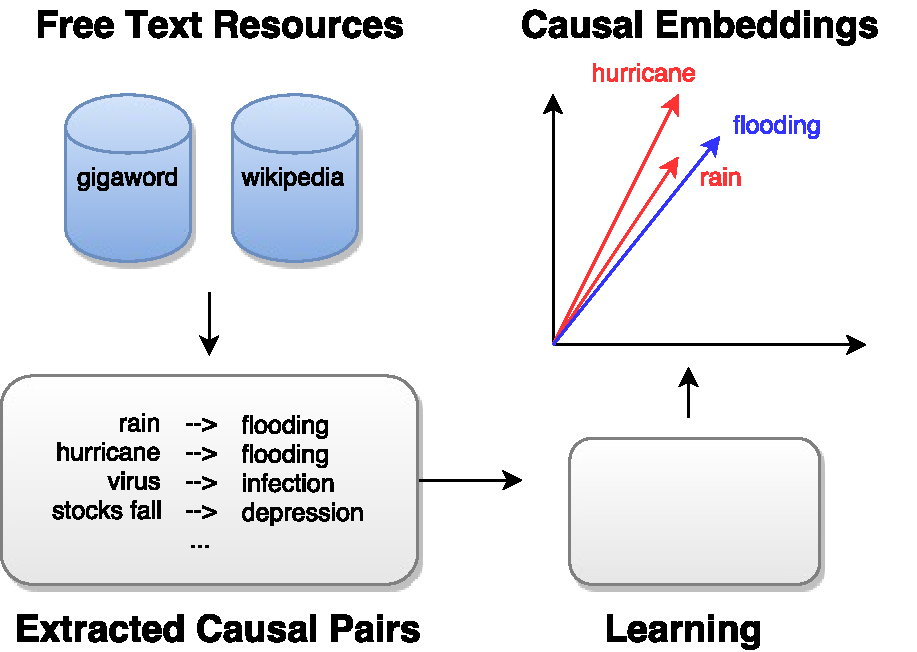
\includegraphics[width=75mm]{emnlpArchDraft.pdf}
%%\vspace{-4mm}
%\caption{{\small Our proposed pipeline for training a causal embedding space from free text resources. \todo{fill in learning with final model}}}
%\vspace{-6mm}
%\label{fig:arch}
%\end{center}
%\end{figure}
%
\section{Approach}
\label{sec:approach}
%\vspace{-2mm}

Our focus is on reranking answers to causal questions using using task-specific distributional similarity methods.
%on the the task of question answering, which is complicated by the variety of question types (e.g., definitional, causal),  each having different information needs that potentially require dedicated solving methods~\cite{clark2013study}.  
%Longer term, we propose a QA approach which uses dedicated, task-specific word embeddings for each question type, aimed at maintaining the robustness of word embeddings while gaining the specificity of dedicated solving methods. 
%Here, we address one particular information need: causality.
%
Our approach operates in three steps:

{\flushleft (1)} We start by bootstrapping a large number of cause-effect pairs from free text using a small number of syntactic and surface patterns (Section \ref{sec:causalextraction}).

{\flushleft (2)} We then use these bootstrapped pairs to build several task-specific embedding (and other distributional similarity) models (Section \ref{sec:models}). We evaluate these models directly on a causal-relation identification task (Section \ref{sec:directeval}).  

{\flushleft (3)} Finally, we incorporate these models into a reranking framework for causal QA and demonstrate that the resulting approach performs better than the reranker without these task-specific models, even if trained on the same data (Section ~\ref{sec:indirecteval}).  


%We approach the task of creating and evaluating a task-specific relational vector space by considering one relation in particular -- causality.  The architecture of our system is shown in Figure \ref{fig:arch}. \todo{do I really need an architecture here?}

%rule-based framework which analyzes free text and returns cause-effect tuples.  
%These pairs are then used to learn a set of high-dimensional word embeddings which are particular to the desired relation.  
%In particular, we make use of the Levy and Goldberg extension of the skipgram algorithm to learn embeddings from these pairs by predicting the effect-text given the cause-text.
%MOVE:
%using the extension of the Skipgram algorithm~\todo{cite and link} proposed by \citep{levy2014dependency}.  
%\todo{does this belong here? intro?}
%While the learning algorithm returns two distinct vector space embeddings for each item in the vocabulary, often only the target embeddings are ever used.  In this work, however, we make use of both sets of embeddings to capture the inherent \emph{directionality} of the causal relation.

%\todo{remove the evaluation info from here?}
%Once trained, we then evaluate the quality this mapping, or vector space, in two ways.  First, we evaluate it directly by attempting to rank a set of cause-effect pairs higher than entity pairs from other relations.  Second, we evaluate the mapping indirectly, by using it in the down-stream task of question answering (QA).



\section{Extracting Cause-Effect Tuples}
\label{sec:causalextraction}
%\vspace{-2mm}

%Information extraction (IE) systems which are designed to extract events typically make use of either machine learning (ML) or hand-built rules or patterns.  %IE classifiers which use ML are generally considered to be either fully supervised (trained only on annotated data), semi-supervised (trained on a combination of labelled data and the data which is bootstrapped from it or by using a large database of pre-known event tuples), or unsupervised (when no labelled data is available for training).
%For causal events, we have neither labelled data nor an existing, large database of cause-effect pairs from which we could use ML to train a supervised or semi-supervised classifier.  Additionally, while unsupervised or distant supervision approaches are well-suited to situations where the desired event types and the patterns that would identify them are unknown, here we know exactly what relation we want (causality) and the patterns needed to find these events are relatively explicit.  For these reasons, we opted to use boostrapping to extract a large number of cause-effect pairs from a small set of patterns.

Because the success of embedding models depends on large training datasets \cite{sharp2015spinning}, and such datasets do not exist for open-domain causality, we opted to bootstrap a large number of cause-effect pairs from a small set of patterns.
%
We wrote these patterns using Odin~\cite{valenzuela2016runes}, a rule-based information extraction framework which has the distinct advantage of 
being able to operate over multiple representations of content (i.e., surface and syntax).
%being \emph{expressive}.  That is, while most open-source rule languages operate over one representation of text (e.g., GATE~\cite{Cunningham2011a} generally operates over surface sequences, whereas Semgrex~\cite{chambers2007learning} operates over syntactic dependencies), Odin has the flexibility to use either (or both) depending on the user's need.  
For this work, we make use of rules that operate over both surface sequences as well as dependency syntax in the grammars introduced in steps (2) and (3) below.

Odin operates as a cascade, % of grammars, 
allowing us to implement a two-stage approach.
%. Taking advantage of this architecture, we implemented a two-stage approach.
First, we identify potential participants in causal relations, i.e., the potential causes and effects, which we term {\bf causal mentions (CM)}. A second grammar then identifies actual causal relations that take these CMs as arguments.

We consider both noun phrases (NP) as well as entire %non-causal
clauses to be potential CMs, since causal patterns form around participants that are syntactically more complex than flat NPs.  
%For example, in the sentence \emph{The hurricane caused significant damage}, both the cause ({\em hurricane}) and effect ({\em damage}) are non-recursive noun phrases.  On the other hand, 
For example, in the sentence \emph{The collapse of the housing bubble caused stock prices to fall}, both the cause ({\em the collapse of the housing bubble}) and effect ({\em stock prices to fall}) are more complicated nested structures.  Reducing these arguments to non-recursive NPs (e.g., {\em The collapse} and {\em stock prices}) is clearly insufficient to capture the relevant context.

%Examples of the rules to extract CMs as well as causal events are shown in Table \ref{tab:rule_examples}\todo{rule examples table}, 

%\begin{table}[t!]
%\begin{center}
%%\begin{scriptsize}
%\begin{footnotesize}
%\begin{tabular}{ll}
%\hline
%\multicolumn{1}{l}{ Rule } & \multicolumn{1}{l}{Example Sentence} \\ %\multicolumn{1}{l}{Impr.} \\
%%\cline{1-2}
%
%\hline
%%\multicolumn{2}{l}{\textit{Yahoo! Answers}} \\ % 185q (sent) ret=1p c=0.1 
%%\hline
%			  &  	\\
%			& 	\\
%	  		& 	\\
%			& 	\\
%
%\end{tabular}
%\end{footnotesize}
%\caption{{\small caption}}
%\label{tab:rules}
%\end{center}
%\end{table}



Formally, we extract our causal relations using the following algorithm:
{\flushleft \textbf{(1) Pre-processing:}} Much of the text we use to extract causal relation tuples comes from the Annotated Gigaword \cite{napoles2012annotated}.  This text is already fully annotated and no further processing is necessary.  We additionally use text from the Simple English Wikipedia\footnote{{\scriptsize \url{https://simple.wikipedia.org/wiki/Main_Page}}.  The Simple English version was preferred over the full version due to its simpler sentence structures, which make extracting cause-effect tuples more straightforward.}, which we processed using the Stanford CoreNLP toolkit~\cite{Manning:14} and the dependency parser of Chen and Manning~\citeyear{chen14}.

{\flushleft \textbf{(2) CM identification:}} \label{step:cm} We extract causal mentions (which are able to serve as arguments in our causal patterns) using a set of rules % (shown in Table \ref{tab:cm_rules}) 
designed to be robust to the variety that exists in natural language. %, and therefore in the dependency parses.  
Namely, to find CMs that are noun phrases, we first find words that are tagged as nouns, then follow outgoing dependency links for modifiers and attached prepositional phrases\footnote{The outgoing dependency links from the nouns which we followed were: \texttt{nn, amod, advmod, ccmod, dobj, prep\_of, prep\_with, prep\_for, prep\_into, prep\_on, prep\_to}, and \texttt{prep\_in}.}, to a maximum depth of two links.  To find CMs that are clauses, we first find words that are tagged as verbs (excluding verbs which themselves were considered to signal causation\footnote{The verbs we excluded were: \emph{cause, result, lead, create}.}), then again follow outgoing dependency links for modifiers and arguments.  We used a total of four rules to label CMs.%\footnote{The two complete grammars, for both CM and causal relation identification, were submitted as supplemental material. \todo{This is no longer relevant. Please remove.}}
%There were a total of four rules used to label CMs, and examples are shown in Table~\ref{tab:rules}.

{\flushleft \textbf{(3) Causal tuple extraction:}} \label{step:causalext} After CMs are identified, a grammar scans the text for causal relations that have CMs as arguments.  Different patterns have varying probabilities of signaling causation~\cite{khoo1998automatic}.  To minimize the noise in the extracted pairs, we restrict ourselves to a set of 13 rules designed to find unambiguously causal patterns, such as {\em CAUSE led to EFFECT}, where {\em CAUSE} and {\em EFFECT} are CMs.
The rules operate by looking for a \emph{trigger} phrase, e.g., {\em led}, and then following the dependency paths to and/or from the trigger phrase to see if all required CM arguments exist.
%, which tells the rule to fire.  Once a trigger is found, the rule follows the dependency paths to and/or from the trigger phrase to see if all specified arguments exist, e.g.,  following an outgoing {\tt nsubj} to identify the cause in the previous example.
%An example of this is shown in Figure \ref{fig:rule_ex}. Here, when the rule scans the sentence \emph{SENTENCE TEXT}, the trigger verb \emph{cause} is found, then the rule checks for an outgoing \texttt{nsubj} dependency link and an outgoing \texttt{dobj} link to previously found CMs.  
%%Our grammars also ensure that the triggers are not negated (we used Odin lookaround assertions to check that outgoing \texttt{neg} dependencies are not attached to triggers).  % Since in this example, all conditions are met, the rule returns the causal event in the form of the tuple (\todo{example}).

% ms: removed for space
%At step~2, the identification of CMs, we place few restrictions on the CM syntactic subgraph, favoring recall since in step 3 we use high-precision rules.  The rule set for step \ref{step:causalext}, in fact, was winnowed down after early experiments showed that many patterns which \emph{can} indicate causation (e.g., {\em X happened due to Y}) often are non-causal (\todo{example}).  

\begin{table}[t!]
\begin{center}
%\begin{scriptsize}
\begin{footnotesize}
\begin{tabular}{lc}
\hline
Corpus		&	Extracted Tuples		 \\
\hline
%\multicolumn{2}{l}{\textit{Yahoo! Answers}} \\ % 185q (sent) ret=1p c=0.1 
%\hline
Annotated Gigaword	& 798,808 	\\
Simple English Wikipedia		& 16,425 	\\
\hline
Total		& 815,233 	\\
\end{tabular}
\end{footnotesize}
\caption{{\footnotesize Number of causal tuples extracted from each corpus.}} 
\label{tab:causalstats}
\vspace{-4mm}
\end{center}
\end{table}

%ltw_mar30_combo.argsC: 55882
%nyt_mar30_combo.argsC: 260460
%wpb_mar30_combo.argsC: 7522
%apw_mar30_combo.argsC: 219348
%xin_mar30_combo.argsC: 76183
%simpleWiki_mar19b_combo.argsC: 14057
%cna_mar30_combo.argsC: 7913
%afp_mar30_combo.argsC: 133003
%sum: 774368

Applying this causal grammar over Gigaword and Simple English Wikipedia produced %774,368 casual tuples, after stop-word and part-of-speech filtering.
815,233 causal tuples, as summarized in Table~\ref{tab:causalstats}. As bootstrapping methods are typically noisy, we manually evaluated the quality of approximately 250 of these pairs selected at random.  Of the tuples evaluated, approximately 44\% contained some amount of noise. For example, from the sentence \emph{Except for Springer's show, which still relies heavily on confrontational topics that lead to fistfights virtually every day...}, while ideally we would only extract (\emph{confrontational topics $\rightarrow$ fistfights}), instead we extract the tuple (\emph{show which still relies heavily on confrontational topics} $\rightarrow$ \emph{fistfights virtually every day}), which contains a large amount of noise: \emph{show, relies, heavily}, etc.
%\todo{Add one example here that is approximately wrong, that is, has some causality but is not ideal. This is to emphasize that, minimally, our tuples capture dist. sim.} 
This finding prompted our noise-aware model described at the end of Section~\ref{sec:models}.

%While this limiting of the rules greatly improved the quality of the extracted causal events, there is still a considerable amount of noise in the data -- a problem we discuss and address in Section \ref{sec:noise} \todo{noise section}. 



\section{Models}
\label{sec-emnlp2016:models}

We use the extracted causal tuples to train three distinct distributional similarity models that explicitly capture causality. 

{\flushleft \textbf{Causal Embedding Model (cEmbed):}}
The first distributional similarity model we use is based on the skip-gram word-embedding algorithm of Mikolov et al.~\citeyear{mikolov2013distributed}, which has been shown to improve a variety of language processing tasks % \footnote{Chris Manning recently called embedding models the Sriracha sauce of NLP.} 
including QA~\cite{yih13,fried2015higher}.  In particular, we use the variant implemented by Levy and Goldberg~\citeyear{levy2014dependency} which modifies the original algorithm to use an arbitrary, rather than linear, context. 
Our novel contribution is to make this context task-specific: intuitively, the context of a cause is its effect. Further, these contexts are generated from tuples that are themselves bootstrapped, which minimizes the amount of supervision necessary.

The Levy and Goldberg model trains using single-word pairs, while our CMs could be composed of multiple words.  
For this reason, we decompose each cause--effect tuple, $(CM_c,CM_e)$, such that each word $w_c \in CM_c$ is paired with each word $w_e \in CM_e$. 

%so we decompose each cause--effect tuple, $(CM_c,CM_e)$, where each CM could be multi-word, into the Cartesian product of the words in CMs. such that each $w_c \in CM_c$ has as its context all $w_e \in CM_e$. 
After filtering the extracted cause-effect tuples for stop words and retaining only nouns, verbs, and adjectives, we generated over 3.6M $(w_c, w_e)$ word-pairs\footnote{For all models proposed in this section we used lemmas rather than words.} from the approximately 800K causal tuples.

The model learns two embedding vectors for each word, one for when the word serves as a target word and another for when the word serves as a context word.  Here, since the relation of interest is inherently directional, both sets of embeddings are meaningful, and so we make use of both -- the target vectors encode the effects of given causes, whereas the context vectors capture the causes of the corresponding effects. 


{\flushleft \textbf{Causal Alignment Model (cAlign):}}
Monolingual alignment (or translation) models have been shown to be successful in QA \cite{Berger:00,Echihabi:03,Soricut:06,Riezler:etal:2007,Surdeanu:11,yao2013}, and recent work has shown that they can be successfully trained with less data than embedding models~\cite{sharp2015spinning}. 
% Further, Fried et al.~\citeyear{fried2015higher} demonstrated that \todo{dest. distribution as semantic model of the source concept, which is important for our task as well.} % ms: nice, but no space

To verify these observations in our context, we train an alignment model that ``translates'' causes (i.e., the ``source language'') into effects (i.e., the ``destination language''), using our cause--effect tuples. 
This is done using IBM Model 1~\cite{Brown:93} and GIZA++~\cite{och03}. 
%We train an alignment model from our cause--effect tuples using  IBM Model 1~\cite{Brown:93} and GIZA++~\cite{och03}.


\begin{figure}[t!]
\begin{center}
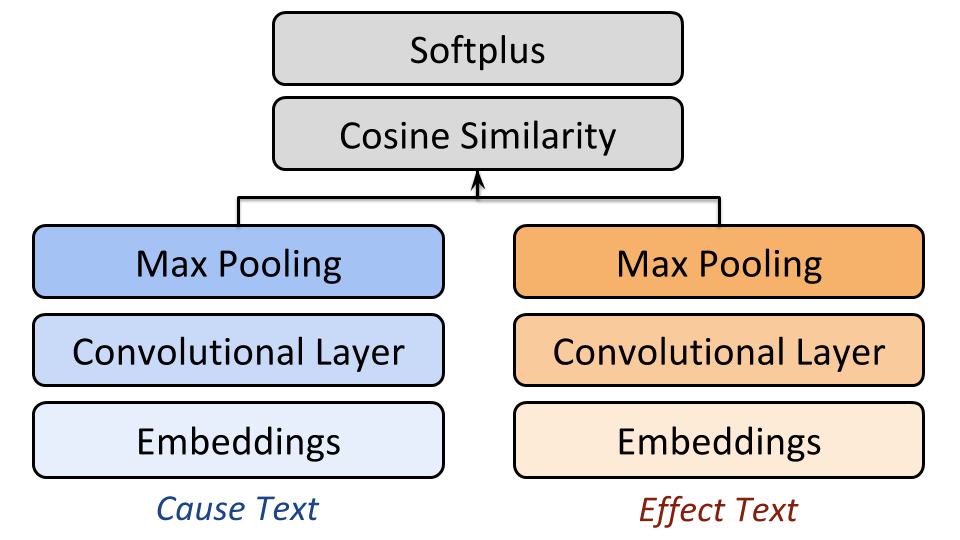
\includegraphics[width=0.7\textwidth]{mainmatter/emnlp2016-causal/cnn2.png}
%space{-2mm}
\caption{{\footnotesize Architecture of the causal convolutional network. }}
%space{-6mm}
\label{fig:cnn}
\end{center}
\end{figure}

{\flushleft \textbf{Causal Convolutional Neural Network Model (cCNN):}}
Each of the previous models have at their root a bag-of-words representation, which is a simplification of the causality task. To address this potential limitation, we additionally trained a convolutional neural network (CNN) which operates over variable-length texts, and maintains distinct embeddings for causes and effects.  The architecture of this approach is shown in Figure~\ref{fig:cnn}, and consists of two sub-networks (one for cause text and one for effect text), each of which begins by converting the corresponding text 
% (which has been padded to be of equal  length)  % ms: skip for now, until we understand it better
into 50-dimensional embeddings.  These are then fed to a convolutional layer,\footnote{The convolutional layer contained 100 filters, had a filter length of 2 (i.e., capturing bigram information), and an inner ReLU activation.} which is followed by a max-pooling layer of equal length.
Then, these top sub-network layers, which can be thought of as a type of phrasal embedding, are merged by taking their cosine similarity.  Finally, this cosine similarity is normalized by feeding it into a dense layer with a single node which has a softplus activation.  
In designing our CNN, we attempted to minimize architectural and hyperparameter tuning by taking inspiration from Iyyer et al.~\citeyear{iyyer2015deep}, preferring simpler architectures.
We train the network using a binary cross entropy objective function and the Adam optimizer~\cite{kingma2014adam}, using the Keras library~\cite{chollet2015keras} operating over Theano~\cite{2016arXiv160502688short}, a popular deep-learning framework.\footnote{We also experimented with an equivalent architecture where the sub-networks are implemented using long short-term memory (LSTM) networks~\cite{hochreiter1997long}, and found that they consistently under-perform this CNN architecture. Our conjecture is that CNNs perform better because LSTMs are more sensitive to overall word order than CNNs, which capture only local contexts, and we have relatively little training data, which prevents the LSTMs from generalizing well.}

{\flushleft \textbf{Noise-aware Causal Embedding Model (cEmbedNoise):}} 
We designed a variant of our cEmbed approach to address the potential impact of the noise introduced by our bootstrapping method.
While training, we weigh the causal tuples by the likelihood that they are truly causal, which we approximate with pointwise mutual information (PMI).
For this, we first score the tuples by their causal PMI and then scale these scores by the overall frequency of the tuple~\cite{riloff1996automatically}, to account for the PMI bias toward low-frequency items.  That is, the score $S$ of a tuple, $t$, is computed as: 

%space{-2mm}
%\scalebox{1.0}{
\begin{small}
\begin{equation}
S(t) = \log \frac{p(tuple|causal)}{p(tuple)} * \log (freq(tuple))
\end{equation} 
\end{small}
%}
%space{-2mm}

%Riloff~\citeyear{riloff1996automatically} propose a method for ranking their extracted patterns using $relevance\_rate * \log_2 (frequency)$.  As our relevance rate we use the pointwise mutual information of the extracted tuples, or $\log \frac{p(tuple|causal)}{p(tuple)}$, where $p(tuple| causal)$ is the ratio of the number of times that a given tuple is found in a causal construction versus any construction, and $p(tuple)$ is the frequency of the given tuple divided by the frequency of all the tuples. 
%Scaling the PMI by the frequency of the tuple mitigates its bias towards low-frequency items.
%we combine PMI with frequency information, so that we consider the likelihood of a pair to be causal to be:
%$p(causal|pair)$ \cite{riloff1996automatically}.
We then discretize these scores into five quantiles, ascribing a linearly decreasing weight during training to datums in lower scoring quantiles.%\footnote{\textcolor{blue}{We implemented this weighing process by repeating higher weight training examples more times.}}



\section{Direct Evaluation: Ranking Word Pairs}

\begin{figure*}[th!]
\begin{center}
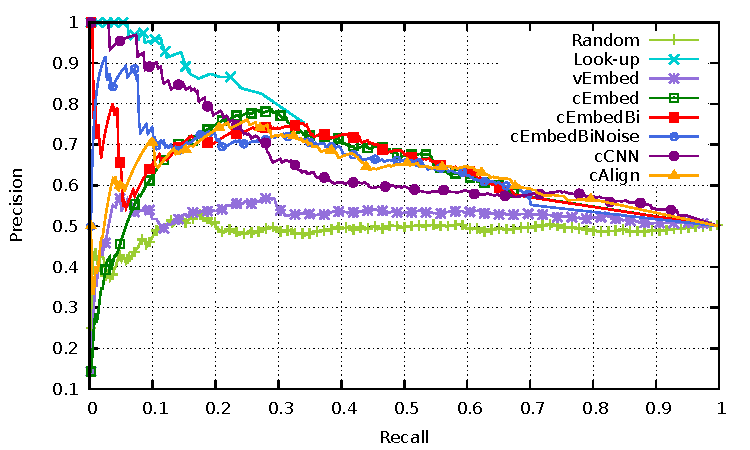
\includegraphics[width=\textwidth]{mainmatter/emnlp2016-causal/direct2.pdf} % {rpcurves_all.png}
%space{-3mm}
\caption{{\footnotesize Precision-recall curve showing the ability of each model to rank causal pairs above non-causal pairs. For clarity, we do not plot cEmbedNoise, which performs worse than cEmbedBiNoise. The Look-up model has no data points beyond the 35\% recall point.}}
%space{-4mm}
\label{fig:rpcurve_all}
\end{center}
\end{figure*}

%\flushleft{\textbf{Results:}} 

\label{sec-emnlp2016:directeval}

%Before we discuss the utility of these models for causal QA, we implement a {\em direct} evaluation
We begin the assessment of our models with a {\em direct} evaluation to determine whether or not the proposed approaches capture causality better than general-purpose word embeddings and whether their robustness improves upon a simple database look-up.
For this evaluation, we follow the protocol of Levy and Goldberg~\citeyear{levy2014dependency}.  
In particular, we create a collection of word pairs, half of which are causally related, with the other half consisting of other relations. 
These pairs are then ranked by our models and several baselines, with the goal of ranking the causal pairs above the others. 
The embedding models rank the pairs using the cosine similarity between the target vector for the causal word and the context vector of the effect word.  The alignment model ranks pairs using the probability $P(\text{Effect}|\text{Cause})$ given by IBM Model 1, and the CNN ranks pairs by the value of the output returned by the network.
%To demonstrate that their embeddings encoded functional similarity rather than relatedness, they ranked a set of word pairs (each of which reflected one of the two types of similarity) using cosine similarity and showed that the word pairs which were functionally similar tended to be ranked higher than those with topical similarity.  Here, we do the same.

%\flushleft{\textbf{Data:}} 
\subsection{Data}
In order to avoid bias towards our extraction methods, we evaluate our models on an external set of word pairs drawn from the SemEval 2010 Task 8 \cite{hendrickx2009semeval}, originally a multi-way classification of semantic relations between nominals.  We used a total of 1730 nominal pairs, 865 of which were from the Cause-Effect relation (e.g., (\emph{dancing $\rightarrow$ happiness})) and an equal number which were randomly selected from the other eight relations (e.g., (\emph{juice $\rightarrow$ grapefruit}), from the Entity-Origin relation).  This set was then randomly divided into equally-sized development and test partitions.

%\flushleft{\textbf{Baselines:}} 
\subsection{Baselines}
We compared our distributional similarity models against three baselines:

{\flushleft \textbf{Vanilla Embeddings Model (vEmbed):}} a standard \texttt{word2vec} model trained with the skip-gram algorithm and a sliding window of 5, using the original texts from which our causal pairs were extracted.\footnote{All embedding models analyzed here, including this baseline and our causal variants, produced embedding vectors of 200 dimensions.} As with the cEmbed model, SemEval pairs were ranked using the cosine similarity between the vector representations of their arguments.
%space{-1mm}

{\flushleft \textbf{Look-up Baseline:}} a given SemEval pair was ranked by the number of times it appeared in our extracted cause-effect tuples. 
%space{-1mm}

{\flushleft \textbf{Random:}} pairs were randomly shuffled.
%space{-1mm}



%%
%% MAP Table 
%%
%\begin{table}[t!]
%\begin{center}
%%\begin{scriptsize}
%\begin{footnotesize}
%\begin{tabular}{ll}
%\hline
%\multicolumn{1}{l}{ Model } & \multicolumn{1}{l}{MAP} \\ %\multicolumn{1}{l}{Impr.} \\
%%\cline{1-2}
%\hline
%%\multicolumn{2}{l}{\textit{Yahoo! Answers}} \\ % 185q (sent) ret=1p c=0.1 
%%\hline
%Random 			& 48.8 	\\
%Look-up			& 63.1$^*$ 	\\
%vEmbed 			& 52.5	\\
%cEmbed  			& 60.8$^*$	\\
%cEmbedBi	                & 62.8$^*$	\\
%cEmbedNoise           & 62.0$^*$	\\ 
%cEmbedBiNoise        & 63.6$^*$	\\ 
%cAlign  			& 61.6$^*$  \\
%cCNN  			& 67.5$^*$	\\
%\end{tabular}
%\end{footnotesize}
%\caption{{\footnotesize Performance in the direct evaluation, measured with mean average precision (MAP).  The ``Bi'' suffix indicates a bidirectional model; the ``Noise'' suffix indicates a model that is noise aware. $^*$  indicates that the difference between the corresponding model and vEmbed is statistically significant ($p < 0.05$), %. Statistical significance was 
%as determined through a one-tailed bootstrap resampling test with 10,000 iterations.}} 
%\label{tab:MAP}
%\vspace{-4mm}
%\end{center}
%\end{table}
%%MAP for Custom Vectors: 0.6816675505751166
%%MAP for E2C Vectors: 0.6871338630607531
%%MAP for Bidir Vectors: 0.6684350003582593
%%MAP for Comparison (Baseline) Vectors: 0.5835158858435683
%%MAP for Translation Model with lamda of 0.5 : 0.6156522257806402
%%MAP for counting Matches: 0.9312613087523468
%%MAP for Keras: 0.6752727545259546
%%MAP for Random: 0.4892479543525109
%%p < 0.01


\subsection{Results}

Figure \ref{fig:rpcurve_all} shows the precision-recall (PR) curve for each of the models and baselines. 
As expected, the causal models are better able to rank causal pairs than the vanilla embedding baseline (vEmbed), which, in turn, outperforms the random baseline.  Our look-up baseline, which ranks pairs by their frequency in our causal database, shows a high precision for this task, but has coverage for only 35\% of the causal SemEval pairs.
%This demonstrates that it is beneficial to have custom models for the semantic relation of interest. 
%First, all the proposed models perform better than the vanilla embedding baseline (vEmbed), which, in turn, outperforms the random baseline. 
%The difference between all our proposed causal models and the vEmbed baseline is statistically significant. 
%

Some models perform better on the low-recall portion of the curve (e.g., the look-up baseline and cCNN), while the embedding and alignment models have a higher and more consistent performance across the PR curve. We hypothesize that models that better \emph{balance} precision and recall will perform better in a real-world QA task, which may need to access a given causal relation through a variety of lexical patterns or variations. We empirically validate this observation in Section~\ref{sec-emnlp2016:indirecteval}.

%, suggesting that causal embedding models may be more practical in a real-world QA system than cCNN. We empirically validate this intuition in Section. 

%perform better in the mid-low recall portion of the curve (e.g. cEmbedBi).  This is well-illustrated by the look-up baseline, which has high precision in the low-recall portion of the curve, but which only has coverage of 35\% of the causal SemEval pairs.  
%The cCNN model outperforms the cEmbed and cAlign models for the low-recall part of the curve (which explains why cCNN has the highest overall MAP). But the latter models 


%Second, the look-up baseline has a higher MAP than several of the causal models, despite having coverage of only 35\% of the causal SemEval pairs.  This suggests that the MAP score is dominated by precision, rather than recall.
%Despite the high overall MAP, this lack of coverage renders this an impractical model, because a real-world QA system is more likely to encounter questions that are lexically different than the pairs in our database. 


%Second, we see that models which had higher MAP demonstrate higher precision in the low-recall portion of the curve, while the models which perform better in the mid-low recall portion of the curve have slightly lower MAPs.  
%This is well-illustrated by the Look-up baseline, whose MAP is higher than many of the causal models, and which has excellent precision in the low-recall portion of the curve, but which only provides coverage for 35\% of the causal pairs.  
%We hypothesize that is the models that better balance precision and recall that will perform well in a real-world QA system, where it is more likely that questions will be lexically different than the pairs in our database.


%Second, somewhat disturbingly, the look-up baseline seemingly outperforms most of the embedding models. 

%However, this score is highly skewed by the fact that approximately 35\% of the causal SemEval pairs were also found in our casual database, and were scored with high precision due to the direct evidence available. However, the remaining pairs received a score of 0. 

%% WHAT IT JUST WAS:
%However, this score is highly skewed: 35\% of the causal SemEval pairs were also found in our casual database, and so were scored with high precision due to the direct evidence available, but the remaining 65\% of pairs all received a score of 0.
%Despite the high overall MAP, this lack of coverage renders this an impractical model, because a real-world QA system is more likely to encounter questions that are lexically different than the pairs in our database. 

%Thus, the MAP score for this model is unrealistically skewed.
% \todo{Say something about how these evaluations are not ideal}~\cite{faruqui2016problems}.

%the high precision of pairs which are found in the database coupled with the very low recall (only 35\% of the pairs were found in the extracted pairs), resulting in the majority of the pairs being tied in the lowest rank, skewing the average.
%that when pairs are found, there is extremely high confidence that they are of the relation of interest coupled with the fact that approximately 65\% of the pairs were not found in the database and so were all tied in last place.  
%As a consequence, there were far fewer average precisions to be combined when calculating the MAP, and most of the ones which were there had extremely high precision.  
% The MAP when using the customized vectors was significantly higher than that of the standard \texttt{word2vec} vectors (68\% versus 58\%, $p<0.01$), and both were higher than the baseline ().  %This suggests that while the standard implementation of \texttt{word2vec} encodes some causality information, our method encodes it far more directly. \todo{better word}.

% \subsection{Discussion}
%To better understand these models, we plot the precision-recall (PR) curve in Figure \ref{fig:rpcurve_all}. 
%The curve highlights the issue discussed above: the look-up model ranks a few pairs with high precision, but does not address the majority of the data. 
%Conversely, the proposed causal models consistently outperform the vEmbed baseline for the high-recall portion of the curve.



The PR curve for the causal embeddings shows an atypical dip at low-recall.  To examine this, we analyzed its top-ranked 15\% of SemEval pairs, and found that incorrectly ranked pairs were not found in the database of causal tuples.  Instead, these incorrect rankings were largely driven by low frequency words whose embeddings could not be robustly estimated due to lack of direct evidence.  
%\todo{Optional: I know we're low on space, but the example that Becky had here was great. Any way to put it back?}
Because this sparsity is partially driven by directionality, 
we implemented a bidirectional embedding model (cEmbedBi) that (a) trains a second embedding model by reversing the input (effects as targets, causes as contexts), and (b) ranks pairs by the \textit{average} of the scores returned by these two unidirectional causal embedding models. 
Specifically, the final bidirectional score of the pair, $(e_1, e_2)$, where $e_1$ is the candidate cause and $e_2$ is the candidate effect, is:
\begin{equation}
s_{bi}(e_1, e_2) = \tfrac{1}{2}(s_{c{\rightarrow}e}(e_1, e_2) + s_{e \rightarrow c}(e_2, e_1))
\end{equation}
where $s_{c \rightarrow e}$ is the score given by the original causal embeddings, i.e., from cause to effect, and $s_{e \rightarrow c}$ is the score given by the reversed-input causal embeddings, i.e., from effect to cause.

As Figure~\ref{fig:rpcurve_all} shows, the bidirectional embedding variants consistently outperform their unidirectional counterparts. 
All in all, the best overall model is cEmbedBiNoise, which is both bidirectional and incorporates the noise handling approach from Section~\ref{sec-emnlp2016:models}. This model substantially improves performance in the low-recall portion of the curve, while also showing strong performance across the curve. 



%
%The curve for the customized vectors shows an atypical shape in its low-recall part.
%Here, the highest ranked pairs had \emph{worse} precision rather than the expected higher precision.  To examine this, we analyzed the top-ranked 15\% of the pairs from the ranking produced by  the causal vectors.  
%%
%Our analysis found that these pairs tend to be incorrectly ranked because the cEmbed model performs a form of soft approximate inference (which was our goal!), but which backfired on these data points.  For example, the top-ranked (incorrect) pair was \emph{platform} $\rightarrow$ \emph{scaffold}, and there were no instances in our causal database where \emph{platform} and \emph{scaffold} were found together in the same cause-effect pair.  
%%
%Instead, we found that there were  three other extracted tuples with \emph{scaffold} in the effect text. Further, these tuples had other effects  that overlapped lexically with effects of \emph{platform}, which ``pulled'' \emph{platform} closer to \emph{scaffold}.  For example, a phrase containing \emph{malfunction} 
%shares {\em loss} as a common effect with \emph{platform}, and \emph{malfunction} has other effects that contain \emph{scaffold}. 
%In general, we found that these examples of semantic drift~\cite{curran2007minimising} occur for low frequency data, where neither the direct evidence nor the embeddings are robustly estimated. 
%
%%cause \emph{loss}, which brings these two words closer in the target embedding space.
%%%, since they have similar effects.  
%%This resulted in \emph{platform}'s effects being close to the effects of \emph{malfunction}, which include \emph{scaffold}.  This demonstrates that the inference is influenced by frequency effects, as words like \emph{scaffold} and \emph{platform} are too infrequent to have robust representations in the embedding space.  
%%\todo{This last sentence needs better explanation: why does this happen only at low-recall?}
%
%As this semantic drift effect is entirely directional, we implemented a bidirectional embedding approach, which: (a) trains a second embedding model by reversing the input, such that the effects served as the targets and the causes were the contexts, and (b) 
%ranks pairs by the average of the scores returned by the two causal embeddings. As Table~\ref{tab:MAP} and Figure~\ref{fig:rpcurve_all} show, the bidirectional embedding variants consistently outperform their unidirectional counterparts. cEmbedBiNoise, which incorporates the noise handling approach from Section~\ref{sec-emnlp2016:models} and is bidirectional, resolves the dip in low-recall part of the curve, and outperforms cCNN for most of the data. 
%
%%As this effect is entirely directional, we trained a set of vectors by reversing the input, such that the effects served as the targets and the causes were the contexts.  The precision-recall curve when using these embeddings to rank the SemEval pairs is shown in Figure \ref{fig:rpcurve_all}, labelled as E2C.  As expected, the curve follows that of the original vectors, as it suffers from the same issues, but with different noisy pairs ranked highly.  We then ranked the SemEval pairs using an average of the scores returned by the two causal embeddings, to mitigate the frequency effects.  That final, bidirectional curve is also shown in Figure \ref{fig:rpcurve_all}.
%%Instead, we found that many of the causal events which whose cause argument contained the word \emph{platform} had effects which overlapped lexically with those whose cause arguments contained the word \emph{malfunction}, and that there w.  To illustrate, consider the following sentences 
%%we had several extracted causal events whose cause contained the word \emph{platform} and whose effect contained the words \emph{}
%


\vspace{-1mm}
\section{Indirect Evaluation: QA Task}
\vspace{-1mm}
%\label{sec:qa}
\label{sec:indirecteval}

%\todo{Describe the QA system and its features shortly, in 1 paragraph.}
The main objective of our work is to investigate the impact of a customized causal embedding model for QA. Following our direct evaluation, which solely evaluated the degree to which our models directly encode causality, here we evaluate each of our proposed causal models in terms of their contribution to a downstream real-world QA task.

Our QA system uses a standard reranking approach~\cite{jansen14}.
%To evaluate the contribution of each of our causal models for QA, we use a standard reranking approach~\cite{jansen14}.
In this architecture, the candidate answers are initially extracted and ranked using a shallow candidate retrieval (CR) component that uses solely information retrieval techniques, then they are re-ranked using a ``learning to rank'' approach.
In particular, we used SVM rank\footnote{ \url{http://www.cs.cornell.edu/people/tj/svm_light/svm_rank.html}}, a Support Vector Machines classifier adapted for ranking, and re-ranked the candidate answers with a set of features derived from both the initial CR score and the models we have introduced. For our model combinations (see Table \ref{tab:QA}), the feature set includes the CR score and the features from each of the models in the combination.
%We compare the performance of our causal models against the same vanilla embeddings model (vEmbed) used in Section \ref{sec:directeval}, the vanilla alignment model (vAlign) of Fried et al.~\citeyear{fried2015higher} trained over the same corpus as the questions,  as well as the look-up baseline.
%

\subsection{Data}

% Our models were trained on open-domain resources, so 
We evaluate on a set of causal questions extracted from the Yahoo! Answers corpus\footnote{Freely available through Yahoo!'s Webscope
program ({\scriptsize {\tt research-data-requests@yahoo-inc.com}})} with simple surface patterns such as \emph{What causes ...} and ~\emph{What is the result of ...}\footnote{We lightly filtered these with stop words to remove non-causal questions, such as those based on math problems and the results of sporting events. Our dataset will be freely available, conditioned on users having obtained the Webscope license.}.
%As we trained our embeddings using events extracted from open-domain resources, we chose to   
We extracted a total of 3031 questions, each with at least four candidate answers, and we evaluated performance using five-fold cross-validation, with three folds for training, one for development, and one for testing. 
%\todo{details about the avg num answers, etc}

\subsection{Models and Features}

We evaluate the contribution of the bidirectional and noise-aware causal embedding models (cEmbedBi, and cEmbedBiNoise) as well as the causal alignment model (cAlign) and the causal CNN (cCNN).  These models are compared against three baselines: the vanilla embeddings (vEmbed), the lookup baseline (LU), and additionally a vanilla alignment model (vAlign) which is trained over 65k question-answer pairs from Yahoo! Answers.

The features\footnote{Due to the variety of features used, each feature described here is independently normalized to lie between 0.0 and 1.0.} we use for the various models are:

{ \flushleft \textbf{Embedding model features:}}
For both our vanilla and causal embedding models, we use the same set of features as 
%Sharp et al.~\citeyear{sharp2015spinning} and 
Fried et al.~\citeyear{fried2015higher}: the maximum, minimum, and average pairwise cosine similarity between question and answer words, as well as the overall similarity between the composite question and answer vectors.  
When using the causal embeddings, since the relation is directed, we first determine whether the question text is the cause or the effect\footnote{We do this through the use of simple regular expressions, e.g., "\^~[Ww]hat ([a-z]+ )\{0,3\}cause.+"}, which in turn determines which embeddings to use for the question text and which to use for the candidate answer texts.  For example, in a question such as "\emph{What causes X?}", since \emph{X} is the effect, all cosine similarities would be found using the effect vectors for the question words and the cause vectors for the answer candidate words. 

{\flushleft \textbf{Alignment model features:}} We use the same global alignment probability, $p(Q|A)$ of Surdeanu et al.~\citeyear{Surdeanu:11}. In our causal alignment model, we adapt this to causality as $p(\text{Effect}|\text{Cause})$, and again we first determine the direction of the causal relation implied in the question.  We include the additional undirected alignment features based on Jensen-Shannon distance, proposed more recently by Fried et al.~\citeyear{fried2015higher}, in our vanilla alignment model.  However, due to the directionality inherent in causality, they do not apply to our causal model so there we omit them.

{\flushleft \textbf{Look-up feature:}} For the look-up baseline we count the number of times words from the question and answer appear together in our database of extracted causal pairs, once again after determining the directionality of the questions.  If the total number of matches is over a threshold\footnote{Empirically determined to be 100 matches.  Note that using this threshold performed better than simply using the total number of matches.}, we consider the causal relation to be established and give the candidate answer a score of 1; or a score of 0, otherwise.

%\section{Downstream QA Evaluation}
%\label{sec:indirecteval}

%The main objective of our work is to investigate the impact of problem-specific solving components for QA. 
%Here we focus on causal QA.
% develop dedicated question-answering (QA) system components for specific question types.  We therefore evaluate our causal models, which we previously determined to encode causality (Section \ref{sec:indirecteval}), in a down-stream (QA) task with causal questions. 


\begin{table}[t!]
\begin{center}
%\begin{footnotesize}
\begin{footnotesize}
\begin{tabular}{lll}
\hline
\# & Model & P@1 \\ 
\hline
& Baselines & \\
\hline
1	&	Random 				& 16.43 	\\
2	&	CR					& 24.31	\\
3	&	CR + vEmbed 			& 34.61	\\
4	&	CR + vAlign			& 19.24	\\
5	&	CR + Look-up	 (LU)	& 29.56 	\\
\hline
& Single Causal Models 		& \\
\hline
6	&	CR + cEmbedBi       & 31.32\\
7	&	CR + cEmbedBiNoise  & 30.15 \\ 
8	&	CR + cAlign  		& 23.49 \\
9	&	CR + cCNN  			& 24.66	\\
\hline
& Model Combinations & \\
\hline
10	&	CR + vEmbed + cEmbedBi		& 37.08$^{*}$	\\ %p < 0.001
11	& 	CR + vEmbed + cEmbedBiNoise 	& 35.50$^*$	\\ %p < 0.05
12	&	CR + vEmbed + cEmbedBi + LU	& 36.75$^{*}$	\\ %p < 0.001
13	&	CR + vEmbed + cAlign		& 	34.31 	\\ %if worse, we can remove and just say that it doesn't stack, per Mihai
14	&	CR + vEmbed + cCNN		& 	33.45 \\
\hline
& Model Stacking & \\
\hline
%15	&	CR + vEmbed + cEmbedBi + cEmbedBi$^2$	& 37.22	\\
15	& 	CR + vEmbed + cEmbedBi + cEmbedBiNoise 	& {\bf 37.28$^{*}$}	\\ 

\end{tabular}
\end{footnotesize}
\vspace{-1mm}
\caption{{\footnotesize Performance in the QA evaluation, measured by precision-at-one (P@1).  The ``Bi'' suffix indicates a bidirectional model; the ``Noise'' suffix indicates a model that is noise aware. $^*$  indicates that the difference between the corresponding model and the CR + vEmbed baseline is statistically significant ($p < 0.05$), %. Statistical significance was 
determined through a one-tailed bootstrap resampling test with 10,000 iterations. }} 
\label{tab:QA}
\vspace{-8mm}
\end{center}
\end{table}

\subsection{Results}
The overall results are summarized in Table~\ref{tab:QA}.
Lines 1--5 in the table show that each of our baselines performed better than CR by itself, except for vAlign, suggesting that the vanilla alignment model does not generate accurate predictions for causal questions.
The strongest baseline was CR + vEmbed (line 3), the vanilla embeddings trained over Gigaword, at 34.6\% P@1. For this reason, we consider this to be the baseline to ``beat'', and perform statistical significance of all proposed models with respect to it. 

Individually, the cEmbedBi model is the best performing of the causal models.  While the performance of cAlign in the direct evaluation was comparable to that of cEmbedBi, here it performs far worse (line 6 vs 8), suggesting that the robustness of embeddings is helpful in QA.  Notably, despite the strong performance of the cCNN in the low-recall portion of the PR curve in the direct evaluation, here the model performs poorly (line 9).

No individual causal model outperforms the strong vanilla embedding baseline (line 3), likely owing to the reduction in generality inherent to building task-specific QA models.
However, comparing lines 6--9 vs. 10--14 shows that the vanilla and causal models are capturing different and complementary kinds of knowledge (i.e., causality vs. association through distributional similarity), and are able to be combined to increase overall task performance (lines 10--12).  These results highlight that QA is a complex task, where solving methods need to address the many distinct information needs in question sets, including both causal and direct association relations.  This contrasts with the direct evaluation, which focuses strictly on causality, and where the vanilla embedding baseline performs near chance. This observation highlights one weakness of word similarity tasks: their narrow focus may not directly translate to estimating their utility in real-world NLP applications. % \footnote{Continuing the food analogies initiated by Chris Manning, the direct evaluation is the equivalent of taking vitamin C instead of eating the whole orange (the downstream task).}

%Of the causal models, the highest performing was cEmbedBi, the bidirectional causal embedding model.  
%Additionally, we see that both of the causal embeddings models stack with the vEmbed model (lines 10 and 11).  
Adding in the lookup baseline (LU) to the best-performing causal model does not improve performance (compare lines 10 and 12), suggesting that the bidirectional causal embeddings subsume the contribution of the LU model.  
cEmbedBi (line 10) also performs better than cEmbedBiNoise (line 11). We conjecture that the ``noise'' filtered out by cEmbedBiNoise contains distributional similarity information, which is useful for the QA task.  cEmbedBi vastly outperforms cCNN (line 14), suggesting that strong overall performance across the precision-recall curve better translates to the QA task.  We hypothesize that the low cCNN performance is caused by insufficient training data, preventing the CNN architecture from generalizing well. 

%We see a small increase when we combine both variants of the causal embeddings model (cEmbedBi and cEmbedBiNoise -- line 15), showing that they contribute slightly different information. 
Our best performing overall model combines both variants of the causal embedding model (cEmbedBi and cEmbedBiNoise), reaching a P@1 of 37.3\%, which shows a 7.7\% relative improvement over the strong CR + vEmbed baseline.

% ms: replaced with text above
%Additionally, on the simpler direct evaluation, where the task consisted entirely of determining causality between two words, the causal models were superior to the baselines and seemingly more sufficient for the task.  The QA task, however, is more complex and not purely about determining causality.  Here we need both similarity \emph{and} causality to do well, as demonstrated by the significant improvement gained by stacking the cEmbed model with the vEmbed model.

% this is future work: I propose to skip it due to lack of space? Also, one of our main contribution is that this knowledge acquisition process is implemented independently of the evaluations. This paragraph negates that.
%\todo{discuss the noise variant and its lack of better performance}
%The failure of the noise-aware causal embeddings model to do better on the QA task suggests that the method we employed is not sufficient to the task.  For example, by weighing some examples more highly than others, we are not actually \emph{removing} the noise, only hoping to downplay it.  Additionally, the manner by which we weighed the extracted tuples was entirely disconnected from the training process as well as the down-stream task.  We suspect that learning the quality of the tuples jointly during training~\cite{tibshirani2014robust} might result in more robust task-specific noise-handling.


%\begin{table}[t!]
%\begin{center}
%%\begin{footnotesize}
%\begin{footnotesize}
%\begin{tabular}{ll}
%\hline
%Feature 	& SVM weight \\
%\hline
%CR	&	\\
%vEmbed max similarity		&	0.021\\
%cEmbed max similarity		&	0.828\\
%vEmbed min similarity		&	-1.703\\
%cEmbed min similarity		&	-0.445\\
%vEmbed avg similarity		&	-1.842\\
%cEmbed avg similarity		&	-2.177\\
%vEmbed overall similarity	&	2.867\\
%cEmbed overall similarity	&	1.725\\
%
%\end{tabular}
%\end{footnotesize}
%
%\caption{{\footnotesize SVM weights learned for each of the features in . }} 
%\label{tab:weights}
%\vspace{-8mm}
%\end{center}
%\end{table}

\begin{table}[t!]
\begin{center}
%\begin{footnotesize}
\begin{footnotesize}
\begin{tabular}{ll}
\hline
Error/observation 	& \% Q \\
\hline
Both chosen and gold are equally good answers 	& 	45\% \\ 
%Chosen answer is longer 							&	35\% \\
Causal max similarity of chosen is higher		&	35\% \\
Vanilla overall similarity of chosen is higher	&	35\% \\
Chosen answer is better than the gold answer		&	25\% \\
The question is very short / lacks content words	&	15\%	 \\
Other 											&	10\% \\
\end{tabular}
\end{footnotesize}

\caption{{\footnotesize Results of an error analysis performed on a random sample of 20 incorrectly answered questions showing the source of the error and the percentage of questions that were affected. Note that questions can belong to multiple categories. }} 
\label{tab:ea}
\vspace{-8mm}
\end{center}
\end{table}


\subsection{Error Analysis}
\label{sec:erroranalysis}

We performed an error analysis to gain more insight into our model as well as the source of the remaining errors.  For simplicity, we used the combination model CR + vEmbed + cEmbedBi. Examining the model's learned feature weights, we found that the vanilla overall similarity feature had the highest weight, followed by the causal overall similarity and causal maximum similarity features.  This indicates that even in causal question answering, the overall \emph{topical} similarity between question and answer is still useful and complementary to the causal similarity features.


To determine sources of error, we randomly selected 20 questions that were incorrectly answered and analyzed them according to the categories shown in Table \ref{tab:ea}.  We found that for 70\% of the questions, the answer chosen by our system was as good as or better than the gold answer, often the case with community question answering datasets.


Additionally, while the maximum causal similarity feature is useful, it can be misleading due to embedding noise, low-frequency words, and even the bag-of-words nature of the model (35\% of the incorrect questions).  For example, in the question \emph{What are the effects of growing up with an older sibling who is better than you at everything?}, the model chose the answer \emph{...You are you and they are them - you will be better and different at other things...}  largely because of the high causal similarity between (\emph{grow} $\rightarrow$ \emph{better}).  While this could arguably be helpful in another context, here it is irrelevant, suggesting that in the future improvement could come from models that better incorporate textual dependencies.







%\vspace{-1mm}
\section{Conclusion}
%\vspace{-1mm}
We presented a framework for creating customized embeddings tailored to the information need of causal questions.  We trained three popular models (embedding, alignment, and CNN) using causal tuples extracted with minimal supervision by bootstrapping cause-effect pairs from free text, and evaluated their performance both directly (i.e., the degree to which they capture causality), and indirectly (i.e., their real-world utility on a high-level question answering task). 


%We note that the results of these two evaluations are not identical; higher performance on the direct evaluation does \emph{not} necessarily correlate with higher performance in the QA task.
We showed that models that incorporate a knowledge of causality perform best for both tasks. 
Our analysis suggests that the models that perform best in the real-world QA task are those that have consistent performance across the precision-recall curve in the direct evaluation.
In QA, where the vocabulary is much larger, precision must be balanced with high-recall, and this is best achieved by our causal embedding model.  Additionally, we showed that vanilla and causal embedding models address different information needs of questions, and can be combined to improve performance. 

Extending this work beyond causality, we hypothesize that additional embedding spaces customized to the different information needs of questions would allow for robust performance over a larger variety of questions, and that these customized embedding models should be evaluated both directly and indirectly to accurately characterize their performance. 

%We introduced a methodology for producing causal embedding models cost-effectively by bootstrapping cause-effect pairs extracted from free text using a small set of seed patterns, and then training dedicated embedding models over this data using task-specific contexts, i.e., where the context of a cause is its effect. We then used these causal embedding models to implement a dedicated reranking model for causal QA. 

%We evaluated the generated embedding models both directly, in a word similarity task, and indirectly, in the downstream QA task. Our analysis yielded multiple observations. First, causal embeddings significantly outperform vanilla embeddings in both tasks, demonstrating the importance of having dedicated models for the task at hand. Second, for QA, the causal embeddings stack well with vanilla ones, highlighting that QA is a complex task, where solving methods need to address multiple information needs. Third, we note that the results of these two evaluations are not identical; higher performance on the direct evaluation does not necessarily correlate with higher performance in the QA task. Our analysis suggests that the performance on the direct evaluation is driven by precision, whereas for the real-world QA task, where the vocabulary is much larger, the precision must be balanced with high-recall which is best achieved by our causal embedding model.  

%We hypothesize that additional embedding spaces customized to the different information needs of questions would allow for robust performance over a larger variety of questions, and that these customized embedding models should be evaluated both directly and indirectly to accurately characterize their performance. 

\section*{Resources}
All code and resources needed to reproduce this work are  available at \url{http://clulab.cs.arizona.edu/data/emnlp2016-causal/}.

% ms: removed for anonymous submission
\section*{Acknowledgments}
We thank the Allen Institute for Artificial Intelligence for funding this work.
Additionally, this work was partially funded by the Defense Advanced
Research Projects Agency (DARPA) Big Mechanism
program under ARO contract W911NF-14-1-0395.


\newpage
%\bibliography{emnlp2016}
%\bibliographystyle{emnlp2016}

%\end{document}

% Our packages
%\usepackage{float}
%\usepackage[font=small]{caption}
%\usepackage{color}
%\usepackage{graphicx}
%\usepackage{booktabs}
%\usepackage{subcaption}
%\usepackage{hyperref}
%\usepackage[utf8]{inputenc}
%\usepackage{tabularx}
%\usepackage{tablefootnote}
%\usepackage{amsmath}
%\usepackage{amssymb}
%\usepackage{placeins}
%\usepackage{scrextend}

%\title{Tell Me Why: Using Question Answering as Distant Supervision for Answer Justification}


%\begin{abstract}
%
%For many applications of question answering (QA), being able to explain why a given model chose an answer is critical.  However, the lack of labeled data for  answer justifications makes learning this difficult and expensive.  Here we propose an approach that uses answer ranking as distant supervision for learning how to select informative justifications. 
%We propose a neural network architecture for QA that reranks answer justifications as an intermediate (and human-interpretable) step in answer selection. Our approach is informed by a set of features designed to combine both learned representations and explicit features to capture the connection between questions, answers, and answer justifications.
% We show that with this end-to-end approach we are able to significantly improve upon a strong IR baseline in both justification ranking (+9\% rated highly relevant) and answer selection (+6\% P@1).  %We also provide an error analysis that demonstrates that we can use the justifications returned to better understand what our model has learned.
%\end{abstract}

\chapter{EMNLP2017 - QAJ\label{chapter:emnlp2017}}

\section{Introduction}
\label{sec-emnlp2017:intro}

Developing interpretable machine learning (ML) models, that is, models where a human user can \emph{understand} what the model is learning, is considered by many to be crucial for ensuring usability and accelerating progress \cite{craven1996extracting,Kim2015MindTG, letham2015interpretable, Ribeiro2016WhySI}.  
% bs: removed for space, we talk more about this in related work
%As such, it has received much attention in recent years, especially as deep learning and complex architectures have seen dramatic gains in many tasks.
For many applications of question answering (QA), i.e., finding short answers to natural language questions, simply providing an answer is not sufficient. A complete approach must be interpretable, i.e., able to {\em explain} why an answer is correct. 
For example, in the medical domain, a QA approach that answers treatment questions would not be trusted if the treatment recommendation is not explained in terms that can be understood by the human user. 
%, the need for interpretable models:
%QA is one of the most challenging natural language understanding tasks~\cite{Etzioni:11}.  Adding to this challenge is the fact that, 
%for many applications of QA, simply providing an answer is not sufficient. A complete approach must also {\em explain} why an answer is correct. 
%For example, in the medical domain, a QA approach that answers treatment questions would not be trusted if the treatment recommendation is not explained in terms that can be understood by the human user. 
%Despite the importance of explanatory QA, the task of providing justifications as to \emph{why} the extracted answers are correct often takes a backseat to the accuracy of the system, and is not evaluated.
%is often overlooked and not evaluated. 

One approach to interpreting complex models is to make use of human-interpretable information % metric % ms: not a metric...
 generated by the model to gain insight into what the model is learning.  This can be an intermediate representation used by the model, as with the model-generated text spans of \citet{Lei2016RationalizingNP}, that serve as input to another classification network.  
By learning these intermediate representations end-to-end with a downstream task, they are optimized to correlate with what the model learns is discriminatory for the task, and they can be evaluated against what a human would consider to be important.
%\todo{need to define what a downstream task means to use this term}, they are optimized to correlate with what the model learns is discriminatory for the task, and they can be evaluated against what a human would consider to be important.
Here we apply this general framework for model interpretability to QA.
% ms: redundant with paragraph below
% propose a QA model that is able to provide free-text passages as justifications for the answers it selects.  

\begin{table}[t]
\begin{center}
\begin{footnotesize}
\begin{tabularx}{\linewidth}{p{0.13cm}p{6.8cm}}
\multicolumn{2}{p{8cm}}{\textbf{Question:} Which of these is a response to an internal stimulus?} \\
 (A) & A sunflower turns to face the rising sun. \\
 (B) & A cucumber tendril wraps around a wire. \\
 (C) &  A pine tree knocked sideways in a landslide grows upward in a bend. \\
 (\textbf{D}) &\textbf{Guard cells of a tomato plant leaf close when there is little water in the roots .} \\
\\
\multicolumn{2}{p{7.2cm}}{\textbf{Justification:} 
Plants rely on hormones to send signals within the plant in order to respond to internal stimuli such as a lack of water or nutrients. } \\

\end{tabularx}
\end{footnotesize}
\caption{{  Example of an 8th grade science question with a justification for the correct answer.  Note the lack of direct lexical overlap present between the justification and the correct answer, demonstrating the difficulty of the task of finding justifications using traditional distant supervision methods. }}
%space{-6mm} 
\label{tab:question_example}
\end{center}
\end{table}

In this work, we focus on answering multiple-choice science exam questions (Clark \citeyear{clark:2015}; see example in Table~\ref{tab:question_example}). 
This domain is challenging as: (a) approximately 70\% of science exam question shave been shown to require complex forms of inference to solve \cite{clark:2013,jansen-EtAl:2016:COLING}, and (b) there are few structured knowledge bases to support this inference.  
Within this domain, we propose an approach that learns to both select and explain answers, when the only supervision available is for which answer is correct (but not how to explain it).
%Within this domain, we propose an approach that jointly learns to select and explain answers, when the only supervision available is for which answer is correct (but not how to explain it) 
%\todo{PC's comment was remove reference to joint learning so it doesn't get us into trouble.  Do we need to say that we're learning the QA task while providing latent information for the explanation task?}. 
Intuitively, our approach chooses the justifications that provide the most help towards ranking the correct answers higher than incorrect ones.
More formally, our neural network approach alternates between using the current model with max-pooling to choose the highest scoring justifications for correct answers, and optimizing the answer ranking model given these justifications. %\todo{ms: tried to simplify, please check}
%bs - very good! thanks!
% scores all possible justifications for a chosen answer with the current model, and then uses max-pooling 
% re-ranks supporting textual evidence for a chosen answer then uses max-pooling 
%\todo{first reference to deep learning -- needs to be introduced before hand} 
%to choose the highest scoring justification and assign the score of the top-ranked justification to the answer candidate itself for use in the answer selection.  
%such that \todo{expand a bit; mention max-pooling?}.  
Crucially, these reranked texts serve as our human-readable answer justifications, and by examining them, we gain insight into what the model learned was useful for the QA task.   


The specific contributions of this work are:
\begin{enumerate}
\item We propose an end-to-end neural method for learning to answer questions and select a high-quality justification for those answers. 
Our approach re-ranks free-text answer justifications without the need for structured knowledge bases. 
%We formulate this such that the answer ranking supervises the justification re-ranking. 
With supervision only for the correct answers, % but not the quality of their corresponding justifications, % ms: redundant with previous text
we learn this re-ranking through a form of distant supervision -- i.e., the answer ranking supervises the justification re-ranking. 
%bs: I added detail in body of intro
%\todo{this is not very clear; say explicitly what we do with max pooling? or, actually, probably ok to remove since it's redundant to main body of the intro; better explain it there, and just summarize the novelty here}
%Because in our setup we have supervision only for the correct answers, but not for the corresponding answer justifications, .

\item We investigate two distinct categories of features in this ``little data'' domain: explicit features, and learned representations. % \todo{Deep learning jargon, needs to be introduced} \bs{I mainly diagree... and due to serious lack of space I can't intro... so idk.  mihai?}.  % ms: not necessary; well known in this community
We show that, with limited training, explicit features perform far better despite their simplicity. %\todo{Are they simpler? They were generated by a human carefully considering the data}.
%bs: i think we can support their simplicity --they're based on like, proportion of lexical overlap and IR scores.

\item We demonstrate a large (+9\%) improvement in generating high-quality justifications over a strong information retrieval (IR) baseline, while maintaining near state-of-the-art performance on the multiple-choice science-exam QA task, demonstrating the success of the end-to-end strategy.
%Importantly, our approach explains its selected answers significantly better than  a strong IR baseline, demonstrating the success of the joint strategy.
%We demonstrate near state-of-the-art performance on the multiple-choice science-exam QA task: our system would have placed 7th in a recent Kaggle challenge (top 4\%).\footnote{{\scriptsize \url{https://www.kaggle.com/c/the-allen-ai-science-challenge/leaderboard}}} 
%Further, our approach outperforms a recent model that relies on structured knowledge bases~\citep{khot2017tupleinf}, despite having a minimally-tuned, simple architecture, and a smaller set of text-only resources. 
% ms: I took it out because the natural question is why don't we evaluate on that dataset as well?
%which achieves state-of-the-art performance on a related question set. 
\end{enumerate}



%\todo{remove me later -- had weird splitting citation issue again.......... } 

%\todo{move this para to related work}

%The way we have formulated our justification selection (as a re-ranking of knowledge base sentences) is related to, but distinct from the task of answer sentence selection \cite[][inter alia]{Wang2010ProbabilisticTM, Severyn:12,Severyn:13a,Severyn:13b,Severyn2015LearningTR,wang2015long}.  Answer sentence selection is typically framed as a fully or semi-supervised task for factoid questions, and 
%.  Additionally, even when this isn't the case and a semi-supervised approach is necessary, 
%the problem is designed such that a correctly selected sentence will fully contain the answer text.
%the exact span of the answer is fully contained within the correct sentence.   
%Here, we have a variety of questions, many of which are non-factoid.  Additionally, we also have no direct supervision for our justification selection (i.e., we have no labels as to which sentences are good jutsifications for our answers), requiring a form of distant supervision where the performance on our QA task serves as our only signal as to whether or not we are selecting good jutstifcations.   Further, we are not actually looking for sentences that \emph{contain} the answer choice, as with answer sentence selection, but rather sentences which close the "lexical gap" \cite{Berger:00} between question and answer (as demonstrated in the question in Table \ref{tab:question_example}). 


%
%\todo{choose either ``explanation'' or ``justification'' and be consistent}
%\bs{i vote justification and tried to be consistent -- arguments? I'll leave the todo til the end to make sure we're good} 
%
%Question answering (QA), i.e., finding short answers to natural language questions, is one of the most challenging natural language understanding tasks~\cite{Etzioni:11}. Adding to this complexity is the fact that, for many applications of QA, simply providing an answer is not sufficient. A complete approach must also {\em explain} why an answer is correct. 
%For example, in the medical domain, a QA approach that answers treatment questions would not be trusted if the treatment recommendation is not explained in terms that can be understood by the human user. 
%Despite the importance of explanatory QA, the task of providing justifications as to why the extracted answers are correct is often overlooked and not evaluated. 
%
%In this work we argue that answers and their justifications re-enforce each other, and, thus, answer selection and justification should be addressed jointly.
%%bs: removed -- 2 ppl now think this is a bit of a jump/stretch
%%We see this as an initial step towards explainable artificial intelligence.\footnote{For more details see DARPA's Explainable Artificial Intelligence program: {\scriptsize \url{http://www.darpa.mil/program/explainable-artificial-intelligence}}.}
%In particular, we propose a joint approach to select and explain answers to multiple-choice science exam questions~\todo{cite ai2} by re-ranking supporting evidence in the form of free-text. The domain of science exam questions is challenging as: (a) many questions require natural language inference to be answered (see, for example, the question in Table~\ref{tab:question_example}) and (b) there are few structured knowledge bases to support this inference.  
%
%%Additionally, the task of selecting a justification for an answer in this domain is difficult because unlike in typical answer sentence selection tasks with factoid questions (where answer sentences generally completely contain the answer text)~\todo{cite moschitti}, here there is often a ``lexical chasm''~\cite{Berger:00} between answer choices and their justifications.  Also, answer sentence selection is typically a fully-supervised problem but here we have no labels for good justifications.
%The way we have formulated our justification selection (as a re-ranking of knowledge base sentences) is related to, but distinct from the task of answer sentence selection \cite[][inter alia]{Wang2010ProbabilisticTM, Severyn:12,Severyn:13a,Severyn:13b,Severyn2015LearningTR,wang2015long}.  Answer sentence selection is typically framed as a fully supervised task for factoid questions.  Additionally, even when this isn't the case and a semi-supervised approach is necessary, the problem is designed such that the answer is fully contained within the desired KB sentence.   Here, we have a variety of questions, many of which are non-factoid.  We also have no direct supervision for our justification selection, requiring a form of distant supervision (i.e., our joint-learning approach), and to further complicate the task, we are not specifically looking for sentences that \emph{contain} the answer choice, but rather sentences which close the "lexical gap" \cite{Berger:00} between question and answer (as demonstrated in the question in Table \ref{tab:question_example}). 

%Additionally, the task of selecting a justification for an answer in this domain is difficult because unlike in typical answer sentence selection tasks with factoid questions (where answer sentences generally completely contain the answer text)~\todo{cite moschitti}, here there is often a ``lexical chasm''~\cite{Berger:00} between answer choices and their justifications.  Also, answer sentence selection is typically a fully-supervised problem but here we have no labels for good justifications.

%\todo{reformulate -- our justs may or may not contain the answer - may be lexical chasm... not designed to contain the answer, but to address the lex chasm}


%Intro: Explanatory ML. Not �"black boxes". Here we focus on explainable QA. Selecting correct answers is important, but providing justifications as to why those answers are correct is critical in many domains.  This is often overlooked and not evaluated, and limits the ultimate utility and applicability of these systems.

%What we do: focus on science exam questions. hard for two reasons: ``lexical chasm'' which requires natural language inference to be solved. 
%We propose and evaluate an deep learning based approach that jointly extracts and explains answers. 

\section{Related work}

In many ways, deep learning has become the canonical example of the "black box" of machine learning and many of the approaches to explaining it can be loosely categorized into two types: approaches that try to interpret the parameters themselves (e.g., with visualizations and heat maps \citep{Zeiler2014VisualizingAU,nips15_hermann, Li2016VisualizingAU}, and approaches that generate a human-interpretable metric that is ideally correlated with what is being learned inside the model (e.g., \citet{Lei2016RationalizingNP}). Our approach falls into the latter type -- 
we use our model's reranking of human-readable justifications to give us insight into what the model considers informative for answering questions.  This allows us to see where we do well (Section \ref{sec-emnlp2017:justification_results}), and where we can improve (Section  \ref{sec-emnlp2017:erroranalysis}).

Deep learning has been successfully applied to many recent QA approaches and related tasks \cite[][inter alia]{Bordes2015LargescaleSQ,nips15_hermann, He2016CharacterLevelQA, dong2015question, Tan2016ImprovedRL}.
%are enticing, and for good reason -- many recent approaches to question answering and related tasks have had much success with various deep learning models \cite[][inter alia]{Bordes2015LargescaleSQ,nips15_hermann, He2016CharacterLevelQA, dong2015question, Tan2016ImprovedRL}.  
However, large quantities of data are needed to train the millions of parameters often contained in these models.  
%Of potentially greater utility in low-data domains, 
Recently, simpler model architectures have been proposed that greatly reduce the number of parameters while maintaining high performance \cite[e.g.,][]{Iyyer2015,chen2016thorough,Parikh2016ADA}.  
%For example, \citet{Iyyer2015}'s show that with their Deep Averaged Network, which replaces complex recurrent neural networks with an average of embeddings and a few, albeit large, dense layers, they improved performance on both a sentiment analysis and a QA task.  For natural language inference, \citet{Parikh2016ADA} used a simpler neural alignment  approach with an attention mechanisms to greatly reduce the size of their model while reaching then state-of-the-art performance.  
We take inspiration from this trend and propose a simple neural architecture for our task to offset the limited available training data. 

Another way to mitigate sparse training data is to include higher-level explicit features.  Like \citet{sachan2016science}, we make use of explicit features alongside features from distributed representations to capture connections between questions, answers, and supporting text.  However, we use a simpler set of features and while they use structured and semi-structured knowledge bases, we use only free-text.  %Additionally, though we also learn to select support from our knowledge base (in some ways similar to \citeauthor{sachan2016science}'s latent answer-entailing structure), since we are explicitly trying to perform \emph{explainable} question answering, here we evaluate the justifications learned by our approach and show that they are significantly better than a  strong IR baseline (Section \ref{sec-emnlp2017:justification_results}).   

Our approach to learning justification reranking end-to-end with answer selection is similar to the \citet{jansen2017framing} latent reranking perceptron,  which also operates over free text.  However, our approach does not require decomposing the text into an intermediate representation, allowing our technique to more easily extend to larger textual knowledge bases.  
%ir approach is able to aggregate information from a variety of sources into one justification, our light-weight approach however, does not rely on a large set of heuristics and heavy pre-processing to transform free-text into a structured knowledge base.  

The way we have formulated our justification selection (as a re-ranking of knowledge base sentences) is related to, but distinct from the task of answer sentence selection \cite[][inter alia]{Wang2010ProbabilisticTM, Severyn:12,Severyn:13a,Severyn:13b,Severyn2015LearningTR,wang2015long}.  Answer sentence selection is typically framed as a fully or semi-supervised task for factoid questions, where a correctly selected sentence fully contains the answer text.
%and the problem is designed such that a correctly selected sentence will fully contain the answer text.
Here, we have a variety of questions, many of which are non-factoid.  Additionally, we have no direct supervision for our justification selection (i.e., no labels as to which sentences are good justifications for our answers), motivating our distant supervision approach where the performance on our QA task serves as supervision for selecting good justifications.  Further, we are not actually looking for sentences that \emph{contain} the answer choice, as with answer sentence selection, but rather sentences which close the "lexical chasm" \cite{Berger:00} between question and answer (demonstrated in the example in Table \ref{tab:question_example}). 


%Related work: QA, multiple choice, kaggle challenge, explanation-centered inference, model-specific work (NNs, etc)

%Latest QA papers (latest trends, attn, etc)
%Inspired by this literature (cite DAN \& SNLI, simpler better), but we add this latent layer they don’t have (justification quality). For simple archs: see Danqi Chen at ACL 2016 (similar to DAN but for reading comprehension). 

%Attention models (ACL 2016). Simple especially when you don’t have enough data.

%(visualizations vs analysis of embeddings VS correlated metric EMNLP paper, etc -- interpreting wts if DL is impossible, rather, find correlations betw those and explanatory natural language)

 
%\todo{Add a paragraph comparing against the task of answer sentence selection (see that reviewer from CL, and all those kernel-based papers by Moschitti). The difference is that in our case the answer and its justification arrive from different sources (i.e., the answer is provided in the multiple-choice exam, whereas the justification is extracted from study guides), whereas in previous answer sentence selection work the answer is included in the sentence. In our case we have to deal with bigger ``lexical chasm'' between question/answer/justification.}

%\todo{Discriminative information retrieval for question answering sentence selection(Chen and Van-Durme): Presented a method that selects sentences which contain potential answers for questions from a very large corpus (10\^7 sentences, requiring several thousand questions for training). Their results are dramatically better than Lucene across two datasets and several evaluation measures.}
%(Yih et al.,2013; Wang and Manning, 2010; Heilman and Smith, 2010; Yao et al., 2013a) and recently using neural networks (Yu et al., 2014; Severyn and Moschitti,2015; Wang and Nyberg, 2015; Yin et al.,2016)

%Answer sentence selection diff because we don't need (or want?) complete answer inclusion.

%Our sentences being selected are unlabeled.

%TAG paper!!! 

\begin{figure}[t]
\begin{center}
\includegraphics[width=0.3\textwidth]{arch_overall.png}
\caption{ Architecture of our question answering approach.  
Given a question, candidate answer, and a free-text knowledge base as inputs, we generate a pool of candidate justifications, from which we extract feature vectors.  We use a neural network to score each and then use max-pooling to select the current best justification. This serves as the score for the candidate answer itself.  The red border indicates the components that are trained online. }
\label{fig:arch_overall}
\vspace{-5mm}
\end{center}
\end{figure}

\section{Approach}
\label{sec:approach}
One of the primary difficulties with the explainable QA task addressed here is that, while we have supervision for the correct answer, we do not have annotated answer justifications.  
Here we tackle this challenge by using the QA task performance as supervision for the justification reranking, allowing us to 
%extending a neural QA model to jointly learn both how to 
%jointly 
learn to choose both the correct answer and a compelling, human-readable justification for that answer.

Additionally, similar to the strategy Chen and Manning~\shortcite{chen2014fast} applied to parsing, we combine representation-based features with explicit features that capture additional information that is difficult to model through embeddings, especially with limited training data.
%second contribution is that, similar to the strategy Chen and Manning~\shortcite{chen2014fast} applied to parsing, we combine representation-based features with explicit features that capture additional information that is difficult to model through embeddings.



% ms: avoid "system" too engineering-y
The architecture of our approach is summarized in Figure \ref{fig:arch_overall}.  
Given a question and a candidate answer, we first query an textual knowledge base (KB) to retrieve a pool of potential justifications for that answer candidate.  
For each justification, we extract a set of features designed to model the relations between questions, answers, and answer justifications based on word embeddings, lexical overlap with the question and answer candidate, discourse, and information retrieval (IR) (Section \ref{sec:features}).
These features are passed into a simple neural network to generate a score for each justification, given the current state of the model.  A final max-pooling layer selects the top-scoring justification for the candidate answer and this max score is used also as the score for the answer candidate.  
The system is trained using correct-incorrect answer pairs with a pairwise margin ranking loss objective function to enforce that the correct answer be ranked higher than any of the incorrect answers. 

%The key here is that we use the current state of the model to select the best justification for a given answer candidate from a pool of many candidate justifications.  To do this, we modify the training procedure such that at the start of each epoch \todo{minibatch instead of epoch?}, we first compute a forward pass with each candidate justification to find the top-scoring justification for each candidate answer.
%For a given question, answer candidate, and justification, we combine features based on word embeddings, lexical overlap, discourse, and information retrieval (IR) together in a simple neural architecture to generate a score for the answer candidate.    We then use this selected justification to calculate our gradients for updating the model parameters.  

With this end-to-end approach, the model learns to select justifications that allow it to correctly answer questions.  We hypothesize that this approach enables the model to indirectly learn to choose justifications that provide good explanations as to why the answer is correct. We empirically test this hypothesis in Section \ref{sec:results}, where we show that indeed the model learns to correctly answer questions, as well as to select high-quality justifications for those answers. 
% ms: misleading; it reads as if answer selection is better than IR
% better than a strong IR baseline. 


\begin{figure}[t]
\begin{center}
\includegraphics[width=0.5\textwidth]{ArchDiagram.png}
\caption{ Detailed architecture of the model's scoring component.  
The question, candidate answer, and justification %\edit{(previously obtained through max-pooling)}
% bs: no - the max pooling happens at the end, after the scoring. 
 are encoded (by summing their word embeddings) to create vector representations of each. These representations are combined in several ways to create a set of representation-based similarity features that are concatenated to additional explicit features capturing lexical overlap, discourse and IR information and fed into a feed-forward neural network.  The output layer of the network is a single node that represents the score of the justification candidate.}  %\todo{Take out? As described in Section \ref{sec:approach}, we then use max-pooling over these justification scores to assign a score to the answer candidate itself.} }
 %bs: sure -- it's shown in the arch right next door :)
\label{fig:arch}
\vspace{-5mm}
\end{center}
\end{figure}


\section{Model and Features}
\label{sec:pipeline}
%\bs{we're low on space and I'm not sure we really need all the features in table 2... in fact, do we need the table at all? \\similarity features are described in prose, as are discourse features (and example is in sep figure), and IR++ features.  Should we remove the table and move the description of LO features to prose? we could recapture half a column...}.  
% removed table per mihai email
Our approach consists of three main components: (a) the retrieval of a pool of candidate answer justifications (Section \ref{sec:justretrieval}); (b) the extraction of features for each (Section \ref{sec:features}); and (c) the scoring of the answer candidate itself based on this pool of justifications (Section \ref{sec:nn_model}).  The architecture of this latter scoring component is shown in Figure \ref{fig:arch}. 


%\begin{table}[t]
%\begin{center}
%\begin{footnotesize}
%\begin{tabular}{p{0.5cm}p{6.5cm}}
%%\hline
%%Feature  & Description \\ 
%\hline
%\multicolumn{2}{l}{Representation-Based Features (Emb)} \\
%\hline
%\multicolumn{2}{l}{$sim(Q,A)$, $sim(Q,J)$, and $sim(Q,J)$} \\
%  & The pairwise cosine similarities between the question, answer, and justification representations. \\
%\multicolumn{2}{l}{$sim(Q, uniqueJ)$ and $sim(A, uniqueJ)$} \\
%& The cosine similarities between each of the question and answer representations and the representation for the terms in the justification which don't overlap with either. \\
%\multicolumn{2}{l}{$dist(Q + J, A)$} \\
% & The euclidean distance between the sum of the question and justification representations and that of the answer (see Section \ref{sec:features} for motivation and details).\\
%\hline
%\multicolumn{2}{l}{Lexical Overlap Features (LO)} \\
%\hline
%\multicolumn{2}{l}{\emph{qCoverage}, \emph{aCoverage}, and \emph{qaCoverage}} \\
% & The proportion of question words, of answer words, and of the combined set of question and answer words that also appear in the justification. \\
%% & The proportion of answer words that also appear in the justification. \\
%% & The proportion of combined question and answer words that also appear in the justification. \\ 
%\multicolumn{2}{l}{\emph{jNovelty}} \\
% & The proportion of justification words that do not appear in either the question or the answer. \\
%\multicolumn{2}{l}{\emph{numWords}} \\
% & Length of the justification in words.\tablefootnote{We normalized this value by the maximum justification length.} \\
%
%\hline
%\multicolumn{2}{l}{Semi-Lexicalized Discourse Features (lexDisc)} \\
%\hline
%\multicolumn{2}{l}{\emph{lexDisc$_0$, ..., lexDisc$_n$}} \\
% & A set of indicator-like features that capture the presence of semi-lexicalized discourse relations (see Section \ref{sec:features} for details and example). \\
% \hline
%\multicolumn{2}{l}{IR-Based Features (IR$^{++}$)} \\
%\hline
%\multicolumn{2}{l}{\emph{IR$_{max}$, IR$_{sum}$}} \\
% & \todo{details} \\
%\multicolumn{2}{l}{\emph{IR$_{max}^{boosted}$, IR$_{sum}^{boosted}$}} \\
% & \todo{details} \\
%
%%\hline
%%\multicolumn{2}{l}{Other} \\
%%\hline
%\end{tabular}
%\end{footnotesize}
%\vspace{-1mm}
%\caption{{\footnotesize Summary of the features calculated for each candidate justification.  
% }} 
%\label{tab:feature_examples}
%\end{center}
%\end{table}

\subsection{Candidate Justification Retrieval}
\label{sec:justretrieval}
The first step in our process is to use standard information retrieval (IR) methods to retrieve a set of candidate justifications for each candidate answer to a given question.  To do this, we build a bag-of-words (BOW) query using the content lemmas for the question and answer candidate, boosting the answer lemmas to have four times more weight\footnote{We empirically found this answer term boosting to ensure retrieval of documents which were relevant to the particular answer candidate.}.  We used Lucene\footnote{\url{https://lucene.apache.org}} with a \emph{tf-idf} based scoring function to return the top-scoring documents from the KB.  Each of these indexed documents consists of a single sentence from our corpora, and serves as one potential justification.  
%\todo{Say here that each Lucene document indexes one potential justification, i.e., one sentence from X, or one paragraph from Y?}

\subsection{Feature Extraction}
\label{sec:features}
For each retrieved candidate justification, we extract a set of features based on (a) distributed representations of the question, candidate answer, and justification terms; (b) strict lexical overlap; (c) discourse relations present in the justification; and (d) the IR scores for the justification.

{ \flushleft{\bf Representation-based features (Emb):}} To model the similarity between the text of each question ($Q$), candidate answer ($A$), and candidate justification ($J$), we include a set of features that utilize distributed representations of the words found in each.
%\todo{Needs to explain where the justification vector comes from (e.g. answer passage from IR model)} 
%bs: I disagree -- I think it's pretty clear from 4.1 above.  I added "text" above to make it clearer.  sorry - but we have no space!!!
First we encode each 
%we make a single vector representation for each of the question ($Q$), answer candidate ($A$), and justification ($J$) 
by summing the vectors for each of their words.\footnote{While this BOW approach is not ideal in many ways, it performed equivalently to far more complicated approaches such as LSTMs and GRUs, also noted by \cite{Iyyer2015}, likely due to the limited training data in this domain.}.  We then compute $sim(Q, A)$, $sim(Q, J)$, and $sim(A, J)$ using cosine similarity.  Using another vector representation of only the \emph{unique} words in the justification, i.e., the words that do not occur in either the question or the candidate answer, we also compute $sim(Q, uniqueJ)$ and $sim(A, uniqueJ)$.  

To create a feature which captures the relationship between the question, answer, \emph{and} justification, we take inspiration from TransE, a popular relation extraction framework \citep{Bordes2013TranslatingEF}.  TransE is based on the premise that if two entities, $e_1$ and $e_2$ are related by a relation $r$, then a mapping into $k$ dimensions, $m(x) \in \mathbb{R}^k$ can be learned such that $m(e_1) + m(r) \approx m(e_2)$.  Here, we modify this intuition for QA by suggesting that given the vectorized representations of the question, answer candidate, and justification above, $Q + J \approx A$, i.e., a question combined with a strong justification will point towards an answer.  Here we model this as an explicit feature, the euclidean distance between $Q + J$ and $A$, and hypothesize that as a consequence the model will learn to select passages that maximize the quality of the justifications.
%Thus, we calculate a feature which is the euclidean distance between $Q + J$ and $A$.  Our intuition is that a question combined with a strong justification will point towards an answer.  Here we model this as an explicit feature, and hypothesize that as a consequence the model will learn to select passages that maximize the quality of the justifications.
This makes a total of six features based on distributed representations. %\todo{This is an important theoretical idea, and should be explicitly stated. e.g. (Our intuition is that a question combined with a strong justification will point towards an answer.  Here we model this as an explicit feature, and hypothesize that as a consequence the model will learn to select passages that maximize the quailty of the justifications.)}  

{\flushleft{\bf Lexical overlap features (LO):}} 
%\todo{This is not a great name, because the next features are also explicit... Maybe, lexical overlap features} 
We additionally characterize each justification in terms of a simple set of explicit features designed to capture the size of the justification, as well as the lexical overlap (and difference) between the justification and the question and answer candidate.  We include these five features: the proportion of question words, of answer words, and of the combined set of question and answer words that also appear in the justification; the proportion of justification words that do not appear in either the question or the answer; and the length of the justification in words.\footnote{We normalized this value by the maximum justification length.} 
%The full set of LO features are shown in Table \ref{tab:feature_examples}.

{\flushleft{\bf Semi-Lexicalized Discourse features (lexDisc):}}  These features use the discourse structure of the justification text, which has been shown to be useful for QA~\cite{jansen14,sharp-EtAl:2015:NAACL-HLT, sachan2016science}. %, to generate a set of explicit discourse features.  

We use the discourse parser of \citet{Surdeanu:15} to fragment the text into elementary discourse units (EDUs) and then recursively connect neighboring EDUs with binary discourse relations.
%which is based on the architecture of \citet{hernault10} and \citet{feng12}.  This parser first parses each justification into its elementary discourse units (EDUs) and then recursively connects neighboring EDUs together, assigning each a binary discourse relation label such as \emph{Elaboration} or \emph{Contrast}. Each of these discourse relations consists of a head, a relation label, and a modifier.  
%
For each of the 18 possible relation labels, we create 
a set of semi-lexicalized discourse features that indicate the presence of a given discourse relation as well as whether or not the head and modifier texts contain words from the question and/or the answer.  %This is similar to the discourse-based features of \citet{sachan2016science}, which were the concatenation of the question word (i.e., \emph{why} or \emph{how}) to the relation labels of background sentences.   

For example, for the question \emph{Q: What makes water a good solvent...?  A: strong polarity}, with a discourse-parsed justification [{\em Water is an efficient solvent}]$_{e1}$ [{\em because of this polarity.}]$_{e2}$, we create the semi-lexicalized feature \emph{Q}\_\emph{cause}\_\emph{A}, because there is a {\em Cause} relation between EDUs $e1$ and $e2$, $e1$ overlaps with the question, and $e2$ overlaps with the answer.
%For example, for the justification [{\em Water is an efficient solvent}]$_{e1}$ [{\em because of this polarity.}]$_{e2}$, we create the semi-lexicalized feature \emph{Q\_cause\_A}, because there is a {\em Cause} relation between EDUs $e1$ and $e2$, $e1$ overlaps with the question ({\em What makes water a good solvent...?}), and $e2$ overlaps with the answer ({\em strong polarity}).
Since there are 18 possible discourse relation labels, and the prefix and suffix can be any of \emph{Q, A, QA} or \emph{None}, this creates a set of 288 indicator features.

%\begin{figure}[t]
%\begin{center}
%\includegraphics[width=0.5\textwidth]{DiscourseExample.png}
%\caption{Example showing the discourse feature extracted from a question, answer, and justification.}
%\label{fig:discourseexample}
%\vspace{-5mm}
%\end{center}
%\end{figure}
%
%Consider the example in Figure \ref{fig:discourseexample}, where the justification contains a \emph{Cause} relation whose head contains question words (shown in blue) and whose modifier contains answer words (shown in green).  This corresponds to the semi-lexicalized feature \emph{Q\_cause\_A}.  Since there are 18 possible discourse relation labels, and the prefix and suffix can be any of \emph{Q, A, QA} or \emph{None}, this creates a set of 288 indicator features\footnote{In practice these features can be greater than 1.0.  We wanted to maintain the indicator-like quality of the features while still capturing if a given justification contains several of a certain type of discourse feature.  Thus, we use the fourth-root of the count of each of the discourse features present in the justification as the feature value.}, though in practice many combinations are never found.

{\flushleft{\bf IR-based features (IR$^{++}$):}} 
%\todo{rework in consideration of query details above}
Finally, we also use a set of four IR-based features which are assigned at the level of the answer candidate (i.e., these features are identical for each of the candidate justifications for that answer choice).   
%Given a question and answer candidate, we query the IR system with the content lemmas from both.  
Using the same query method as described in Section \ref{sec:justretrieval}, for each question and answer candidate we retrieve a set of indexed documents.
Using the \emph{tf-idf} based retrieval scores of these returned documents, 
$s(d_i)$ for $d_i \in D$, we rank the answer candidates using two methods: 
\begin{itemize}
\item by the maximum retrieved document score for each candidate, and  
\item by the weighted sum of all retrieved document scores\footnote{Weighted sum was based on the IR scores used in the winning Kaggle system from user Cardal (\scriptsize{ \url{https://github.com/Cardal/Kaggle_AllenAIscience}})}:
\begin{footnotesize}
\vspace{-5mm}
\begin{equation}
\sum_{d_i \in D} \dfrac{1}{i} s(d_i) 
\end{equation}
\vspace{-7mm}
\end{footnotesize} 
\end{itemize}
We repeat this process using an unboosted query as well, for a total of four rankings of the answer candidates.  
We then use these rankings to make a set of four reciprocal rank features,  IR$^{++}_0$, ..., IR$^{++}_3$, for each answer candidate (i.e., IR$^{++}_0 = 1.0$ for the top-ranked candidate in the first ranking,  IR$^{++}_0 = 0.5$ for the next candidate, etc.)
%For each answer candidate, we use its position in each of the four rankings above to make a reciprocal rank feature -- these are the IR$^{++}$ features. 
  
%For each of these four IR-based rankings of the answer candidates, We transform these four IR-based rankings into a set of four reciprocal rank features for each answer candidate. 


\subsection{Neural Network}
\label{sec:nn_model}

As shown in Figure \ref{fig:arch}, the extracted features for each candidate justification are concatenated and passed into a fully-connected feed-forward neural network (NN).  The output layer is a single node representing the justification score.  We then use max-pooling over these scores to select the current best justification for the answer candidate, and use its score as the score for the answer candidate itself.  For training, the correct answer for a given question is paired with each of the incorrect answers, and each are scored as above.  We compute the pair-wise margin ranking loss for each training pair:
\vspace{-2mm}

\begin{footnotesize}
\begin{equation}
L = \max(0, m - F(a^{+}) + F(a^{-}))
\end{equation}
%\vspace{-2mm} 
\end{footnotesize}where $F(a^+)$ and $F(a^-)$ are the model scores for a correct and incorrect answer candidate and $m$ is the margin, and backpropagate the gradients.
At testing time, we use the trained model to score each answer choice (again using the maximum justification score) and select the highest-scoring.

As we are interested in not only correctly answering questions, but also selecting valid justification for those answers, we keep track of the scores of \emph{all} justifications and use this information to return the top $k$ justifications for each answer choice.  These are evaluated along with the answer selection performance in Section \ref{sec:results}.

\section{Experiments}
\label{sec-emnlp2017:experiments}

\subsection{Data and Setup}
We evaluated our model on the set of 8th grade science questions that was provided by the Allen Institute for Artificial Intelligence (AI2) for a recent Kaggle challenge.  The training set contained 2,500 question, each with 4 answer candidates.  For our test set, we used the 800 publicly-released questions that were used as the validation set in the actual evaluation.\footnote{The official testing dataset is not publicly available.}  We tuned our model architectures and hyper-parameters on the training data using five-fold cross-validation (training on 4 folds, validating on 1).  During testing, we froze the model architecture and all hyperparameters and re-trained on all the training data, setting aside a random 15\% of training questions to facilitate early stopping. 
%That is, \todo{explain how early stopping works.}  
% sorry mihai -- no room adn it's common practice in DL.  that sai, if a reviewer wants to know, I'm more than happy to address it with a 9th page...

\subsection{Baselines}
In addition to previous work, we compare our model against two strong IR baselines:
%\paragraph{IR Baseline:} For this baseline, we rank answer candidates by the maximum \emph{tf.idf} document retrieval score using an unboosted query of question and answer terms (see Section \ref{sec-emnlp2017:justretrieval} for retrieval details).
%
%\paragraph{IR$^{++}$:}  This baseline uses the same architecture as the full model, as described in Section \ref{sec-emnlp2017:nn_model}, but with only the IR$^{++}$ feature group.

\begin{itemize}
\item \textbf{IR Baseline:} For this baseline, we rank answer candidates by the maximum \emph{tf.idf} document retrieval score using an unboosted query of question and answer terms (see Section \ref{sec-emnlp2017:justretrieval} for retrieval details).

\item \textbf{IR$^{++}$:}  This baseline uses the same architecture as the full model, as described in Section \ref{sec-emnlp2017:nn_model}, but with only the IR$^{++}$ feature group.
\end{itemize}

\subsection{Corpora}
For our pool of candidate justifications (as well as the scores for our IR baselines) we used the corpora that were cited as being most helpful to the top-performing systems of the Kaggle challenge.  These consisted of short, flash-card style texts gathered from two online resources:  about 700K sentences from StudyStack\footnote{{\scriptsize \url{https://www.studystack.com/}}} and 25K sentences from Quizlet\footnote{{\scriptsize \url{https://quizlet.com/}}}.
From these corpora, we use the top 50 sentences retrieved by the IR model as our set of candidate justifications.  All of our corpora were annotated using using the Stanford CoreNLP toolkit~\cite{manning2014stanford}, the dependency parser of Chen and Manning~\citeyear{chen2014fast}, and the discourse parser of \citet{Surdeanu:15}.
% and indexed with \todo{lucene}. 
%\todo{Explain what a ``document'' is for these resources.} 
%\bs{I do that now in Sect 4.1 -- is that sufficient?}

While our model is able to learn a set of embeddings, we found performance was improved when using pre-trained embeddings, and in this low-data domain, fixing these embeddings to not update during training substantially reduced the amount of model over-fitting.   In order to pre-train domain-relevant embeddings for our vocabulary, we used the documents from the StudyStack and Quizlet corpora, supplemented by the newly released Aristo \textsc{mini} corpus (December 2016 release)\footnote{{\scriptsize \url{http://allenai.org/}}}, which contains 1.2M science-related sentences from various web sources.  The training was done using the \texttt{word2vec} algorithm \cite{mikolov10, mikolov13} as implemented by \citet{levy2014dependency}, such that the context for each word in a sentence is composed of all the other words in the same sentence.  We used embeddings of size 50 as we did not see a performance improvement with higher dimensionality.

\subsection{Model Tuning}
The neural model was implemented in Keras \cite{chollet2015keras} using the Theano \cite{2016arXiv160502688short} backend.  For our feed-forward component, we use a shallow neural network that we lightly tuned to have a single fully-connected layer containing 10 nodes, glorot uniform initialization, a $tanh$ activation, and an L2-regularization of 0.1.  We trained with the RMSProp optimizer \citep{rmsprop},  a learning rate of 0.001, 100 epochs, a batch size of 32, and early stopping with a patience of 5 epochs.  Our loss function used a margin of 1.0.  

We experimented with burn-in, i.e., using the best justification chosen by the IR model for the first mini-batches, but found that models without burn-in performed better, indicating that the model benefited from being able to select its own justification.
 
\begin{table}[t!]
\begin{center}
\begin{footnotesize}
\begin{tabular}{llll}
\hline
\# & Model & P@1 Val & P@1 Test \\ 
%\hline
%& Baselines & \\
\hline
1	&	Random 			&			25			&  25	\\
2	&	IR Baseline		&			47.2			&	 47	\\
3	&	IR$^{++}$ 		&			50.7$^{**}$			& 36.35	\\
4 & \citet{Iyyer2015}
%\tablefootnote{Our implementation of the architecture described in the paper, using the same embeddings we used with our model and dense layers of equal dimension to our embeddings.} 
& -- & 32.52\\
5 & \citet{khot2017tupleinf} & -- & 46.17 \\
%\hline
%	&	Our Approach & 	&	\\
\hline
6 & Our approach w/o IR	&	50.54$^*$	& 48.66 \\
%7	&	IR$^{++}$ + EF 					&		53.4$^{**\dagger\dagger}$				& 53.4$^{**}$	\\
%8	&	IR$^{++}$ + EF + lexDisc 	&		53.6$^{**\dagger\dagger}$				& 53.42$^{**\dagger}$ 	\\
7	&	Our approach  &	{\bf 54.0}$^{**\dagger\dagger}$		& {\bf 53.3}$^{**\dagger}$ 	\\
\end{tabular}
\end{footnotesize}
\vspace{-1mm}
\caption{{\footnotesize Performance on the AI2 Kaggle questions, measured by precision-at-one (P@1).  $^*$s  indicate that the difference between the corresponding model and the IR baseline is statistically significant ($^*$ indicates $p < 0.05$ and $^{**}$ indicates $p < 0.001$) and $^{\dagger}$s  indicate significance compared to IR$^{++}$,
%that the difference between the corresponding model and the IR$^{++}$ baseline is statistically significant. %($^\dagger$ corresponds to $p < 0.05$ and $^{\dagger\dagger}$ corresponds to $p < 0.001$).  
All significance values were determined through a one-tailed bootstrap resampling test with 100,000 iterations. }} 
\label{tab:p@1}
\end{center}
\end{table}

\begin{table}[t!]
\begin{center}
\begin{footnotesize}
\begin{tabular}{ll}
\hline
 Ablated Model & P@1 Val \\ 
\hline
 %LO + lexDisc + Emb	&	50.54$^*$ \\
    %Baseline IR$^{++}$ 							&		50.7$^{**}$	\\
	IR$^{++}$ + LO 					&		53.4$^{**\dagger\dagger}$\\
	IR$^{++}$ + LO + lexDisc 	&		53.6$^{**\dagger\dagger}$ \\
    Full Model (IR$^{++}$ + LO + lexDisc + Emb)  &	{\bf 54.0}$^{**\dagger\dagger}$	\\
\end{tabular}
\end{footnotesize}
\vspace{-1mm}
\caption{{\footnotesize Ablation of feature groups results, measured by precision-at-one (P@1) on validation data.  Significance is indicated as in Table \ref{tab:p@1}.}} 
\label{tab:ablation}
\vspace{-5mm}
\end{center}
\end{table}

\section{Results}
\label{sec:results}

Rather than seeking to outperform all other systems at selecting the correct answer to a question, here we aimed to construct a system system that can produce substantially better justifications for why the answer choice is correct to a human user, without unduly sacrificing accuracy on the answer selection task.  Accordingly, we evaluate our system both in terms of it's ability to correctly answer questions (Section \ref{sec:accuracy}), as well as provide high-quality justifications for those answers (\ref{sec:justification_results}).  Additionally, we perform an error analysis (Section \ref{sec:erroranalysis}), taking advantage of the insight the reranked justifications provide into what the model is learning.
% \todo{not sure what this sentence means?}.
% bs: is this clearer?

\subsection{QA Performance}
\label{sec:accuracy}
We evaluated the accuracy of our system as well as the baselines on the held-out 800 set of test questions.  Performance, measured in precision at 1 (P@1)\cite{manning08}, is shown in Table \ref{tab:p@1} for both the validation (i.e., cross validation on training) and test partitions.  Because NNs are sensitive to initialization, each experimental result shown is the average performance across five runs, each using different random seeds.   

The best performing baseline on the validation data was a model using only IR$^{++}$ features (line 3), but its performance dropped substantially when evaluated on test due to the failure of several random seed initializations to learn.  For this reason, we assessed significance of our model combinations with respect to both the IR baseline as well as the IR$^{++}$ (indicated by $^*$ and $^{\dagger}$s, respectively).
%For this reason, we assessed significance of our model combinations with respect to both the IR baseline (indicated by $^*$) as well as the IR$^{++}$ system (indicated by $^{\dagger}$s).

Our full model that combines IR$^{++}$, lexical overlap, discourse, and embeddings-based features, has a P@1 of 53.3\% (line 7), an absolute gain of 6.3\% over the strong IR baseline despite using the same background knowledge.  
% + LO + lexDisc + Emb\todo{use the text description to make it easier for the reader, e.g. (that combines IR++ with lexical overlap, ...}, has a P@1 of 53.3, an absolute gain of 6.3\% over the strong IR baseline despite using the same background knowledge.  

%\subsubsection{Comparison to Previous Work}
%\begin{flushleft}
%{\bf Comparison to Previous Work}
\vspace{-1mm}
%\end{flushleft}
\paragraph{Comparison to Previous Work:}
We compared our performance against another model that achieves state of the art performance on a different set of 8th grade science questions, \textsc{TupleInf}(T+T') \citep{khot2017tupleinf}.  \textsc{TupleInf}(T+T') uses Integer Linear Programming to find support for questions via tuple representations of KB sentences\footnote{Notably, one portion of the tuple KB used was constructed based on a different 8th grade question set than the one we use here.}.
%with structured Open IE \citep{Banko2007OpenIE} tuple representations of both questions and knowledge-base sentences to assess how well a given answer choice is entailed or supported.  
On our test data, \textsc{TupleInf}(T+T') achieves 46.17\% P@1 (line 5). 
%\todo{move back to 1 sigdig?}.  
As this model is independent of an IR component, we compare its performance against our full system without the IR-based features (line 6), whose performance is 48.66\% P@1, an absolute improvement of 2.49\% P@1 (5.4\% relative) despite our unstructured text inputs and the far smaller size of our knowledge base (three orders of magnitude). 

%Notably, their KB used by \citeauthor{khot2017tupleinf} is three orders of magnitude larger than ours.  
%Waterloo -- 280GB, ours is SS+QZ -- 72.5MB

\citet{sachan2016science} also tackle the AI2 Kaggle question set with an approach  that learns alignments between questions and structured and semi-structured KB data.
%They reframe the task as answer entailment and learn alignments between structured and semi-structured KB data and the question-answer hypothesis.  
They use only the training questions (splitting them into training, validation, and testing partitions), supplemented by questions found in online study guides, and report an accuracy of 47.84\%.  By way of a loose comparison (since we are evaluating on different data partitions), our model has approximately 5\% higher performance despite our simpler set of features and unstructured KB.  

We also compare our model to our implementation of the basic Deep-Averaged Network (DAN) Architecture of \citet{Iyyer2015}.  %To ensure a more fair comparison, 
We used the same 50-dimensional embeddings in both models, so with the reduced embedding dimension, we reduced the size of each of the DAN dense layer to 50 as well.  For simplicity, we also did not implement their word-dropout, a feature that they reported as providing a performance boost. Using this implementation, the performance on the test set was 31.50\% P@1.  To help with observed overfitting, we tried removing the dense layers and received a small boost to 32.52\% P@1 (line 4).  
The lower performance of their model, which relies exclusively on latent representations of the data, underscores the benefit of including explicit features alongside latent features in a deep-learning approach for this domain.
%This lower performance demonstrates, again, \todo{change to "The lower performance of their model, which relies on latent representations of the data, underscores the relative importance of including both explicit and latent features in a deep-learning solver"?}. the utility of explicit features alongside latent representations in low-data domains.

In comparison to other systems that competed in the Kaggle challenge, our system comes in in 7th place out of 170 competitors (top 4\%).\footnote{Based on the public leaderboard ({\scriptsize \url{https://www.kaggle.com/c/the-allen-ai-science-challenge/leaderboard}}). The best scoring submission had an accuracy of 59.38\%.  Note that for the systems that participated, this set served as \emph{validation} while for us it was test, and thus it is likely that these scores are slightly overfitted to this dataset, but for us it was blind.  As such this is a conservative comparison, and in reality the difference is likely to be smaller.}  Compared with the systems which disclosed their methods, we use a subset of their corpora and substantially less hyperparameter tuning, and yet we achieve competitive results.  
%\todo{count cardal hyperparameters and add}
%bs - removed hyperparam count todo bc it's not straightforward and we're out of space anyway.
%\todo{add paragraph for DAN}

%\subsection{Feature Ablation}
%\begin{flushleft}
%{\bf Feature Ablation }
\vspace{-2mm}
%\end{flushleft}

\paragraph{Feature Ablation:} To evaluate the contribution of the individual feature groups, we additionally performed an ablation experiment (see Table \ref{tab:ablation}).
Each of our ablated models performed significantly better than the IR baseline on the validation set, including our simplest model, IR$^{++}$+LO.
%\footnote{As we consider the fully ablated IR$^{++}$ to be a baseline, we do not include it here.}.
%, and the version which has the IR-based features removed, LO+lexDisc+Emb.  
   
%The addition of the semi-lexicalized discourse features (lexDisc) did not significantly improve performance over IR$^{++}$+EF, but it did add the stability needed to show significant gains over IR$^{++}$ (compare lines 3 and 5).  
%The addition of the distributional similarity features, which led to our best performing model on the validation data did not improve performance on the test data (line 5), suggesting that while distributional similarity has been shown effective in situations where there is sufficient training data, it struggles to contribute in low-data domains.  Recall that due to over-fitting issues, we fixed our model embeddings, and so while we used domain-specific embeddings, they were not tuned to be task-specific.  We suspect that given more training data we would see much more benefit from these distributional similarity features.


%
% Justification example
%
\begin{table}[t]
\begin{center}
\begin{footnotesize}
%\begin{tabular}{p{1cm}p(6cm}}
\begin{tabularx}{\linewidth}{p{0.7cm}p{6cm}}
\hline
\multicolumn{2}{c}{Question} \\
\hline			
\multicolumn{2}{p{7cm}}{\textbf{Q:} Scientists use ice cores to help predict the impact of future atmospheric changes on climate. Which property of ice cores do these scientists use? } \\
\multicolumn{2}{p{7cm}}{\textbf{A:} The composition of ancient materials trapped in air bubbles} \\
\multicolumn{1}{c}{} & \multicolumn{1}{c}{} \\				
\hline
\multicolumn{1}{l}{Rating} & \multicolumn{1}{c}{Example Justification} \\
\hline			
{\em Good }		&	Ice cores: cylinders of ice that scientist use to study trapped atmospheric gases and particles frozen with in the ice in air bubbles \\
{\em Half }		&	Ice core: sample from the accumulation of snow and ice over many years that have recrystallized and have	trapped air bubbles from previous time periods \\
{\em Topical }	&   Vesicular texture formation [has] trapped air bubbles. \\
{\em Off-topic }	&	Physical change: change during which some properties of material change but ... \\
%\end{tabular}
\end{tabularx}
\end{footnotesize}
\caption{{  Example justifications from the our model and their associated ratings. }} 
\label{tab:justification_examples}
\vspace{-5mm}
\end{center}
\end{table}

\subsection{Justification Performance}
\label{sec:justification_results}
One of our key claims is that our approach addresses the related, but more challenging problem of performing \emph{explainable} question answering, i.e., providing a high-quality, compelling justification for the chosen answer.  To evaluate this claim, we evaluated a random set of 100 test questions that both the IR baseline and our full system answered correctly.  For each question, we assessed the quality of each of the top five justifications.  For IR, these were the highest-scoring retrieved documents, and for our system, these were the top-scoring justifications as re-ranked by our model.  Following the methodology of Jansen et al. \citeyear{jansen2017framing}, each justification received a rating of either \emph{Good} (if the connection between the question and correct answer was fully covered), \emph{Half} (if there was a missing link), \emph{Topical} (if the justification was simply of the right topic), or \emph{Off-Topic} (if the justification was completely unrelated to the question). Examples of each rating are provided in Table \ref{tab:justification_examples}.  

\begin{table}[t]
\begin{center}
\begin{footnotesize}
\begin{tabular}{llll}
\hline
 Model 			& Good@1 	& Good@5 	& NDCG@5 \\ 
\hline
IR Baseline 	&	0.52 		&	0.64 		& 0.55 \\
Our Approach & 	{\bf 0.61}	 	&	{\bf 0.74}			& {\bf 0.62}$^{**}$ \\
\end{tabular}
\end{footnotesize}
\caption{{\footnotesize Percentage of questions that have at least one \emph{good} justification within the top 1 (Good@1) and the top 5 (Good@5) justifications, 
%. returned by both the IR baseline and our full model 
as well as the normalized discounted cumulative gain at 5 (NDCG@5) of the ranked justifications.
 Significance indicated as in Table \ref{tab:p@1}.
% returned by each.  
%For NDCG, $^*$  indicates that the difference was significant ($p < 0.001$)
%, as determined through a 1-tailed bootstrap resampling test with 100,000 iterations.
}} 
\label{tab:justification_ndcg}
\vspace{-5mm}
\end{center}
\end{table}


%\begin{table}[t]
%\begin{center}
%\begin{footnotesize}
%\begin{tabular}{lcc}
%\hline
%% & \multicolumn{5}{c}{\emph{Good}@$k$} \\ 
%Model	& Good@1 & Good@5 \\
%\hline
%IR Baseline 		&	0.52 	&	0.64 \\
%Our Approach 	& 	0.61	 	&	0.74\\
%\end{tabular}
%\end{footnotesize}
%\caption{{\footnotesize Percentage of questions that have at least one \emph{good} justification within the top 1 (Good@1) the top 5 (Good@5) justifications returned by both the IR baseline and our full model.}} 
%\label{tab:justification_performance}
%\end{center}
%\end{table}


%\begin{table}[t]
%\begin{center}
%\begin{footnotesize}
%\begin{tabular}{lccccc}
%\hline
% & \multicolumn{5}{c}{Position Within Top 5} \\ 
%Rating	& 1 & 2 & 3 & 4 & 5\\
%\hline
%\multicolumn{6}{l}{CR Baseline} \\
%\hline
%Good	& 0.52 & 0.42 & 0.39 & 0.35 & \textbf{0.40}\\
%Half		& 0.23 & 0.19 & 0.24 & 0.22 & 0.21\\
%Topical		& 0.18 &0.30 & 0.26 &0.33 & 0.30\\
%Off-Topic	& 0.07 & 0.09 & 0.10 & 0.09 & 0.08\\
%\hline
%\multicolumn{6}{l}{Full Model} \\
%\hline
%Good  &  \textbf{0.61}  &  \textbf{0.54}  &  \textbf{0.43}  &  \textbf{0.40}  &  0.37\\
%Half  &  0.19  &  0.24  &  0.20  &  0.26  &  0.28\\
%Topical  &  0.17  &  0.17  &  0.27  &  0.27  &  0.22\\
%Off-Topic  &  0.02  &  0.05  &  0.09  &  0.06  &  0.12\\
%\end{tabular}
%\end{footnotesize}
%\caption{{\footnotesize Percentage of good, half, topical, and off-topic justifications at each position within the top five justifications returned by both the IR baseline and our full model.}} 
%\label{tab:justification_performance}
%\end{center}
%\end{table}

Results of this analysis are shown using three evaluation metrics in Table \ref{tab:justification_ndcg}.  The first two columns show the percentage of questions which had a \emph{Good} justification at position 1 (Good@1), and within the top 5 (Good@5).  
%justifications with each of the four ratings at each position in the top 5.  
Note that 61\% of the top-ranked justifications from our system were rated as \emph{Good} as compared to 52\% from the IR baseline (a gain of 9\%), despite the systems using identical corpora.  
%In second position, our system had 12\% more \emph{Good} justifications.  

We also evaluated the justification ratings using normalized discounted cumulative gain at 5 (NDCG@5) (as formulated in \citet{manning08}, p.163), where we assigned \emph{Good} justifications a gain of 3.0, \emph{Half} a gain of 2.0, \emph{Topical} a gain of 1.0, and \emph{Off-Topic} a gain of 0.0.  With this formulation, our system had a NDCG@5 of 0.62 while the IR baseline had a significantly lower NDCG@5 of 0.55 ($p < 0.001$), shown in the third column of Table \ref{tab:justification_ndcg}. 

\begin{figure}[t]
\begin{center}
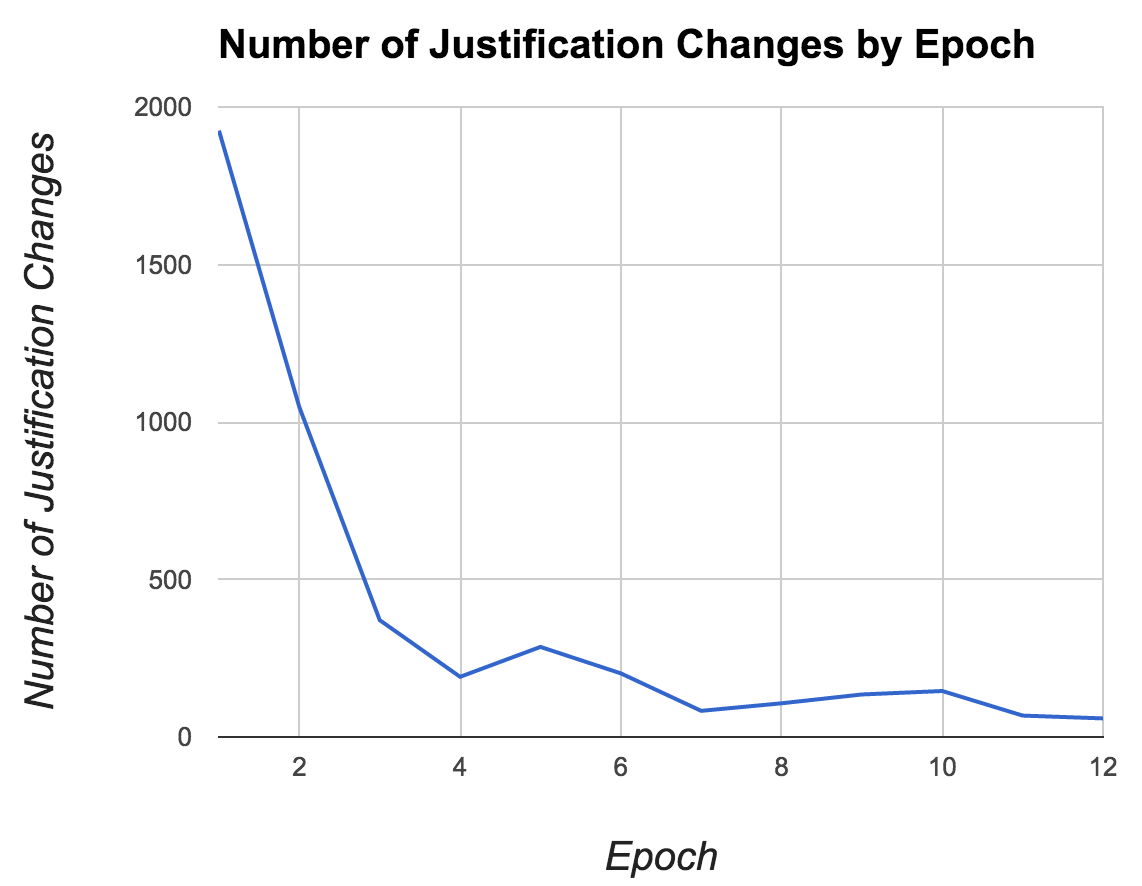
\includegraphics[width=0.8\textwidth]{mainmatter/emnlp2017-qaj/justificationChanges.png}
\caption{Number of questions for which % the IR$^{++}$ + EF + lexDisc + Emb 
our complete model chooses a new justification at each epoch during training.  While this is for a single random seed, we see essentially identical graphs for each random initialization.}
\label{fig:changes}
\vspace{-5mm}
\end{center}
\end{figure}

%\subsection{Contribution of Jointly Learning to Rank Justifications}
%\begin{flushleft}
%{\bf Contribution of Learning to Rerank Justifications}
%\end{flushleft}
\vspace{-2mm}
\paragraph{Contribution of Learning to Rerank Justifications:}
The main assertion of this work is that through learning to rank answers and justifications for those answer candidates in an end-to-end manner, we both answer questions correctly and provide compelling justifications as to why the answer is correct.  To confirm that this is the case, we also ran a version of our system that does not re-rank justifications, but uses the top-ranked justification retrieved by IR.  This configuration dropped our performance on test to 48.7\% P@1, a decrease of 4.6\%, and we additionally lose all justification improvements from our system (see Section \ref{sec:justification_results}), demonstrating that learning this reranking is key to our approach.

Additionally, we tracked the number of times a new justification was chosen by the model as it trained. We found that our system converges to a stable set of justifications during training, shown in Figure \ref{fig:changes}.

%- Demonstrate the need for the latent layer (justifications from IR).


%bs - no room: Greedy is useful: top 1 just vs. top 10 vs. top 100 (OPTIONAL) But we want top 1 anyway.


%\todo{Examples of good/bad questions!?}
%bs: removed todo -- there won't be any room, I promise!

%\todo{Error analysis where it’s doing worse (>= 20+ qs, where our got it wrong) -- 20 questions we got wrong, find top 2 places we went wrong (half a column}

%
%\begin{table}[!th]
%\begin{center}
%\begin{footnotesize}
%\hfill
%\begin{tabular}{ll}
%\hline
%Error Type & Percent \\ 
%\hline
%Short justification/High lexical overlap  & 53.3\%\\
%Complex inference required   & 43.3\% \\
%Knowledge Base Noise  & 6.7\% \\
%Word order necessary	 & 6.7\% \\
%Coverage & 6.7\% \\
%Negation	& 3.3\% \\
%Other & 6.7\% \\
%\end{tabular}
%\end{footnotesize}
%\caption{{\footnotesize Summary of the findings of the 30 question error analysis.  
%%Examples of several categories provided in separate tables. 
%Note that a given question may fall into more than one category.}} 
%\label{tab:erroranalysis}
%\vspace{-5mm}
%\end{center}
%\end{table}
%
%%\begin{table}[!th]
%%\begin{center}
%%\begin{footnotesize}
%%\hfill
%%\begin{tabular}{p{0.8cm}p{6.5cm}p{1cm}}
%%\hline
%%\multicolumn{2}{l}{Error Type} & Percent \\ 
%%\hline
%%\multicolumn{2}{l}{\textbf{Shorter justification with lots of lexical overlap}} & 53.3\%\\
%%\multicolumn{2}{l}{\textbf{Complex inference required}}  & 43.3\% \\
%%\hline
%%
%%\\
%%\hline
%%\multicolumn{2}{l}{\textbf{KB Noise}}  & 6.7\% \\
%%\hline
%%Question: & \multicolumn{2}{p{7.5cm}}{ If an object traveling to the right is acted upon by an unbalanced force from behind it  the object will}	\\
%%Correct: & \multicolumn{2}{p{7.5cm}}{speed up }	\\
%%Chosen & \multicolumn{2}{p{7.5cm}}{ change direction }	\\
%%			& \multicolumn{2}{p{7.5cm}}{\textit{ Unbalanced force: force that acts on an object that will change its direction}}	\\
%%%\hline
%%\multicolumn{3}{p{8cm}}{The system found a sentence in the knowledge base that "justifies" the correct answer.}	\\
%%%
%%\\
%%\hline
%%\multicolumn{2}{l}{\textbf{Word order necessary}}	 & 6.7\% \\
%%\hline
%%Question: & \multicolumn{2}{p{7.5cm}}{ The acceleration of a small rocket that has just been launched can be quantitatively found by}	\\
%%Correct: & \multicolumn{2}{p{7.5cm}}{dividing the force acting upon the rocket by its mass }	\\
%%Chosen & \multicolumn{2}{p{7.5cm}}{ dividing the mass of the rocket by the force acting upon it }	\\
%%			& \multicolumn{2}{p{7.5cm}}{\textit{ (same for both) acceleration: force divided by mass}}	\\
%%%\hline
%%\multicolumn{3}{p{8cm}}{The ordering of the answer choice terms was necessary for answering the question.}	\\
%%%
%%\\
%%\hline
%%\multicolumn{2}{l}{\textbf{Coverage}} & 6.7\% \\
%%\hline
%%Question: & \multicolumn{2}{p{7.5cm}}{ Which activity most effectively ensures the proper functioning of osteocytes?}	\\
%%Correct: & \multicolumn{2}{p{7.5cm}}{consuming mineral-rich foods}\\
%%			& \multicolumn{2}{p{7.5cm}}{\textit{ most lipids consumed from food are in the form of triglycerids}}	\\	
%%Chosen & \multicolumn{2}{p{7.5cm}}{increasing the respiratory rate }	\\
%%			& \multicolumn{2}{p{7.5cm}}{\textit{ hyperventilation increased respiratory rate}}	\\
%%%\hline
%%\multicolumn{3}{p{8cm}}{The knowledge base had no coverage for the concept of \emph{osteocyte}, so the system grasped at proverbial straws.}	\\
%%%
%%\\
%%\hline
%%\multicolumn{2}{l}{\textbf{Negation}}	& 3.3\% \\
%%\hline
%%%\multicolumn{3}{l}{Example}	\\
%%Question: & \multicolumn{2}{p{7.5cm}}{ Which feature does not form as a result of tectonic plates diverging?}	\\
%%Chosen: & \multicolumn{2}{p{7.5cm}}{ rift valley }	\\
%%			& \multicolumn{2}{p{7.5cm}}{\textit{ Rift valley: deep valley formed as tectonic plates move apart. }}	\\
%%\multicolumn{3}{p{8cm}}{Note that the justification actually shows that the chosen answer is incorrect, rather than justifying it.  This is the expected behavior for the system for these negated questions as we don't handle them differently.}	\\
%%%
%%\\
%%\hline
%%\multicolumn{2}{l}{\textbf{Other}} & 6.7\% \\
%%\end{tabular}
%%\hfill
%%\end{footnotesize}
%%\caption{{\footnotesize Summary of the findings of the 30 question error analysis.  Note that a given question may fall into more than one category.}} 
%%\label{tab:erroranalysis}
%%\end{center}
%%\end{table}
%
%\begin{table}[t]
%\begin{center}
%\begin{footnotesize}
%\begin{tabular}{p{1cm}p{6cm}}
%\hline
%Type: & \textbf{Short justification/High lexical overlap}\\
%\hline
%Question: & The length of time between night and day on Earth varies throughout the year. This time variance is explained primarily by $\rule{1cm}{0.15mm}$. \\
%Correct: & Earth 's angle of tilt \\
%			 & \textit{ ... the days are very short in the winter because the sun's rays hit the earth at an extreme angle ... due to the tilt of the earth's axis. } \\
%Chosen: &  Earth 's distance from the Sun \\
%			& \textit{ Is light year time or distance? Distance}	\\
%\end{tabular}
%\hfill
%\end{footnotesize}
%\caption{{\footnotesize Example of the system preferring a justification for which all the terms were found in either the question or answer candidate.
%% while the justification for the correct answer contained additional information necessary to fully explain the answer. 
%(Justifications shown in italics)
%}} 
%\label{tab:ex_lex_overlap}
%\vspace{-5mm}
%\end{center}
%\end{table}
%
%\subsection{Error Analysis}
%\label{sec:erroranalysis}
%
%%\todo{provide examples for all without other -- make full width}
%
%
%To better understand the limitations of our current system, we performed an error analysis of 30 incorrectly answered questions.  %Taking advantage of the ability of the chosen justifications to provide insight into what the system found important, we 
%We examined the top 5 justifications returned for both the correct and chosen answers.  
%%Among the questions analyzed we found some interesting trends.   
%Notably, 50\% of the questions analyzed had one or more good justifications in the top 5 returned by our system, but for a variety of reasons, summarized in Table \ref{tab:erroranalysis}, the system incorrectly ranked another answer's justification higher.  
%
%The most common form of error was the systems preference 
%was when the chosen answer's justification contained a 
%for short justifications with a large degree of lexical overlap with the question and answer choice itself, 
%%with few unmatched terms, 
% shown by the example in Table \ref{tab:ex_lex_overlap}.  
% %This effect was magnified when the correct answer required more "explanation" to connect the question to the answer.  
%This suggests that the system has learned that generally many unmatched words are indicative of an incorrect answer.  While this may typically be true, extending the system to be able to prefer the \emph{opposite} with certain types of questions would potentially help with these errors.  
%
%The second largest source of errors came from questions requiring complex inference (causal, process, quantitative, or model-based  reasoning) as with the question:%.  For example, to answer the question:
% %\begin{quote}
%\begin{addmargin}[1em]{2em}% 1em left, 2em right 
% \begin{footnotesize}
%  \textit{Q: Mr. Harris mows his lawn ...[and leaves] the clippings on the ground. Which long term effect will this most likely have on his lawn? \\
%  A: It will provide the lawn with needed nutrients.}
% \end{footnotesize}
%%\end{quote}
%\end{addmargin}
%To answer this, you would need to link together: \textit{cut grass left on the ground $\rightarrow$ grass decomposes $\rightarrow$ decomposed material provides nutrients}. 
%These questions constitute a large portion of our errors,  
%%is a large set of questions that our system is not particularly designed to handle, 
%demonstrating not only the difficulty of the question set but also the need for systems that can robustly handle a variety of question types and their corresponding information needs.  
%
%Aside from these main groups, there were some smaller trends:  
%7\% of the incorrectly chosen answers actually had justifications which "validated" them due to noise in the knowledge base, 7\% required word-order to answer (e.g., \emph{mass divided by acceleration} vs. \emph{acceleration divided by mass}), another 7\% of questions suffered from lack of coverage of the question concept in the knowledge base,
%%(see example in Table \ref{tab:ex_coverage}), 
% and 3\% failed to appropriately handle negation (i.e., questions of the format \emph{Which of the following are NOT ...}). 
%
%
%
%% bs: no room: - Negative results?


%\begin{table}[t]
%\begin{center}
%\begin{footnotesize}
%\begin{tabular}{p{1cm}p{6cm}}
%\hline
%Type: & \textbf{Coverage}\\
%\hline
%Question: & Which activity most effectively ensures the proper functioning of osteocytes? \\
%Correct: & consuming mineral-rich foods\\
%			& \textit{ most lipids consumed from food are in the form of triglycerids}	\\	
%Chosen & increasing the respiratory rate 	\\
%			& \textit{ hyperventilation increased respiratory rate}	\\
%\end{tabular}
%\hfill
%\end{footnotesize}
%\caption{{\footnotesize Example of a question for which coverage was an issue.  The KB had no coverage for the concept of \emph{osteocyte}.}} % , so the system grasped at proverbial straws.}} 
%\label{tab:ex_coverage}
%\end{center}
%\end{table}


%\begin{table}[!th]
%\begin{center}
%\begin{footnotesize}
%\begin{tabular}{p{1cm}p{6cm}}
%\hline
%Type: & \textbf{Complex inference required}\\
%\hline
%Question: & Mr. Harris mows his lawn twice each month. He claims that it is better to leave the clippings on the ground. Which long term effect will this most likely have on his lawn? \\
%Correct: &  It will provide the lawn with needed nutrients. 	\\
%\end{tabular}
%\hfill
%\end{footnotesize}
%\caption{{\footnotesize Example of a question for which complex inference is required.  In order to answer the question, you would need to assemble the following chain of events: cut grass left on the ground $\rightarrow$ grass decomposes $\rightarrow$ decomposed material provides nutrients.}} 
%\label{tab:ex_complex_inf}
%\end{center}
%\end{table}


%\begin{table}[!th]
%\begin{center}
%\begin{footnotesize}
%\hfill
%\begin{tabular}{ll}
%\hline
%Error Type & Percent \\ 
%\hline
%Short justification/High lexical overlap  & 53.3\%\\
%Complex inference required   & 43.3\% \\
%Knowledge Base Noise  & 6.7\% \\
%Word order necessary	 & 6.7\% \\
%Coverage & 6.7\% \\
%Negation	& 3.3\% \\
%Other & 6.7\% \\
%\end{tabular}
%\end{footnotesize}
%\caption{{\footnotesize Summary of the findings of the 30 question error analysis.  
%%Examples of several categories provided in separate tables. 
%Note that a given question may fall into more than one category.}} 
%\label{tab:erroranalysis}
%\vspace{-5mm}
%\end{center}
%\end{table}


%\begin{table}[t]
%\begin{center}
%\begin{footnotesize}
%\begin{tabular}{p{1cm}p{6cm}}
%\hline
%Type: & \textbf{Short justification/High lexical overlap}\\
%\hline
%Question: & The length of time between night and day on Earth varies throughout the year. This time variance is explained primarily by $\rule{1cm}{0.15mm}$. \\
%Correct: & Earth 's angle of tilt \\
%			 & \textit{ ... the days are very short in the winter because the sun's rays hit the earth at an extreme angle ... due to the tilt of the earth's axis. } \\
%Chosen: &  Earth 's distance from the Sun \\
%			& \textit{ Is light year time or distance? Distance}	\\
%\end{tabular}
%\hfill
%\end{footnotesize}
%\caption{{\footnotesize Example of the system preferring a justification for which all the terms were found in either the question or answer candidate. (Justifications shown in italics)
%}} 
%\label{tab:ex_lex_overlap}
%\vspace{-5mm}
%\end{center}
%\end{table}

\subsection{Error Analysis}
\label{sec-emnlp2017:erroranalysis}

We performed an error analysis of 30 incorrectly answered questions, %summarized in Table \ref{tab:erroranalysis},
  examining the top 5 justifications returned for both the correct and chosen answers of each.    
%Among the questions analyzed we found some interesting trends.   
Notably, 50\% of the questions had one or more \emph{Good} justifications. %, but the system incorrectly ranked another answer's justification higher.  
The most common form of error (53.3\%) was due to the system's preference for short justifications with a large degree of lexical overlap with the question and answer choice, %, particularly when the correct answer required more "explanation" to connect the question to the answer.  
% shown by the example in Table \ref{tab:ex_lex_overlap}.  
 %This effect was magnified when the correct answer required more "explanation" to connect the question to the answer.  
suggesting the system has learned that generally many unmatched words are indicative of an incorrect answer.  %While this may typically be true, extending the system to be able to prefer the \emph{opposite} with certain types of questions would potentially help with these errors.  
The second largest source of errors (43.3\%) came from questions requiring complex inference (causal, process, quantitative, or model-based reasoning), demonstrating the difficulty of the question set and the need for systems that can robustly handle a variety of question types.
Aside from these main groups, there were some smaller trends including KB noise, and our system's lack of using word order and recognizing negation.\footnote{A much more detailed error analysis is available, and if this paper is accepted will be included.}
 
% as with the question:%.  For example, to answer the question:
 %\begin{quote}
%\begin{addmargin}[1em]{2em}% 1em left, 2em right 
% \begin{footnotesize}
%  \textit{Q: Mr. Harris mows his lawn ...[and leaves] the clippings on the ground. Which long term effect will this most likely have on his lawn? \\
%  A: It will provide the lawn with needed nutrients.}
% \end{footnotesize}
%%\end{quote}
%\end{addmargin}
%To answer this, you would need to link together: \textit{cut grass left on the ground $\rightarrow$ grass decomposes $\rightarrow$ decomposed material provides nutrients}. 
%These questions constitute a large portion of our errors,   demonstrating not only the difficulty of the question set but also the need for systems that can robustly handle a variety of question types and their corresponding information needs.  

%Aside from these main groups, there were some smaller trends including:  
%7\% of the incorrectly chosen answers actually had justifications which "validated" them due to KB noise, 7\% required word-order to answer (e.g., \emph{X divided by Y} vs. \emph{Y divided by X}), %another 7\% of questions suffered from lack of coverage of the question concept in the knowledge base,
%%(see example in Table \ref{tab:ex_coverage}), 
% and 3\% failed to appropriately handle negation (i.e., questions of the format \emph{Which of the following are NOT ...}). 


% bs: no room: - Negative results?


%\begin{table}[t]
%\begin{center}
%\begin{footnotesize}
%\begin{tabular}{p{1cm}p{6cm}}
%\hline
%Type: & \textbf{Coverage}\\
%\hline
%Question: & Which activity most effectively ensures the proper functioning of osteocytes? \\
%Correct: & consuming mineral-rich foods\\
%			& \textit{ most lipids consumed from food are in the form of triglycerids}	\\	
%Chosen & increasing the respiratory rate 	\\
%			& \textit{ hyperventilation increased respiratory rate}	\\
%\end{tabular}
%\hfill
%\end{footnotesize}
%\caption{{\footnotesize Example of a question for which coverage was an issue.  The KB had no coverage for the concept of \emph{osteocyte}.}} % , so the system grasped at proverbial straws.}} 
%\label{tab:ex_coverage}
%\end{center}
%\end{table}


%\begin{table}[!th]
%\begin{center}
%\begin{footnotesize}
%\begin{tabular}{p{1cm}p{6cm}}
%\hline
%Type: & \textbf{Complex inference required}\\
%\hline
%Question: & Mr. Harris mows his lawn twice each month. He claims that it is better to leave the clippings on the ground. Which long term effect will this most likely have on his lawn? \\
%Correct: &  It will provide the lawn with needed nutrients. 	\\
%\end{tabular}
%\hfill
%\end{footnotesize}
%\caption{{\footnotesize Example of a question for which complex inference is required.  In order to answer the question, you would need to assemble the following chain of events: cut grass left on the ground $\rightarrow$ grass decomposes $\rightarrow$ decomposed material provides nutrients.}} 
%\label{tab:ex_complex_inf}
%\end{center}
%\end{table}


\section{Conclusion}

Here we propose an end-to-end question answering (QA) model that learns to correctly answer questions as well as provide compelling, human-readable justifications for its answers,  despite not having access to labels for justification quality.  We do this by using the question answering task as a form of distant supervision for learning  justification re-ranking.  We show that our accuracy and justification quality are significantly better than a strong IR baseline, while maintaining near state-of-the-art performance for the answer selection task as well.
% and that  the QA task performance is better than several other baselines.  
%This framework can also be extended to allow the model to learn different priorities for justification selection given different question information needs, which we leave to future work.
%\FloatBarrier


%\section*{Acknowledgments}

%\bibliography{refs}
%\bibliographystyle{emnlp_natbib}
%
%\end{document}


% Include the various appendices
\appendix
\chapter{Sample Appendix\label{apndxA}}

Stuff.....



% Switch the spacing to single-spaced for the references
\renewcommand{\baselinestretch}{1}		% changing the value
\small\normalsize										% switch size to make the value take

% Create the References list
\bibliographystyle{uabibnat}
\bibliography{bibliography}

\end{document}
